\documentclass[utf8, aspectratio=169]{beamer} 

\usepackage[english]{babel}
\usepackage{booktabs} % "schoene" Tabellen ermoeglichen
\usepackage[T1]{fontenc} % interne Font-Generierung
\usepackage[hang]{footmisc} % haengende Fussnoten
\usepackage{graphicx} % Abbildungen ermoeglichen
\usepackage{lmodern} % Schriftfamilie Latin Modern. Als letzten Schrift laden, damit es die aktive ist.
\usepackage{textcomp} % zusaetzliche LaTeX-Sonderzeichen
\usepackage{hyperref} % Hypertextstrukturen ermoeglichen, automatically loaded by beamer
\usepackage[babel]{csquotes} % "schoene" Anfuehrungszeichen
\usepackage{xspace}
\usepackage{amsmath}
\usepackage{amssymb}
\usepackage{mathtools}
\usepackage{xfrac}
\usepackage{siunitx}
\usepackage{dsfont}
\usepackage{tabularx}
\usepackage{caption}
\usepackage{subcaption}
\usepackage{fontawesome5}
\usepackage{placeins}  % \FloatBarrier
\usepackage{exercise}
\usepackage{enumerate}

% Wir wollen Grossbuchstaben für Chapter, Section and Subsection,
% so wie es für Figure, Table, etc. bereits der Default ist.
% Siehe Dokumentation for hyperref.
\addto\extrasenglish{
    \def\chapterautorefname{Chapter}
	\def\sectionautorefname{Section}
	\def\subsectionautorefname{Subsection}
	\def\subsubsectionautorefname{Subsubsection}
	\def\paragraphnameautorefname{Paragraph}
}

\AtBeginEnvironment{definition}{\renewcommand\eminnershape{\bfseries}}

\DeclareMathOperator{\Prob}{\mathbb{P}}
\DeclareMathOperator{\E}{\mathbb{E}}  % alternative: \mathbf{E}
\newcommand{\eps}{\varepsilon}
\newcommand{\R}{\mathbb{R}}
\renewcommand{\P}{\mathbb P}
\newcommand{\bx}{\boldsymbol{x}}
\newcommand{\bX}{\boldsymbol{X}}

% Color in math environments
% https://tex.stackexchange.com/a/261480
\makeatletter
\def\mathcolor#1#{\@mathcolor{#1}}
\def\@mathcolor#1#2#3{%
  \protect\leavevmode
  \begingroup
    \color#1{#2}#3%
  \endgroup
}
\makeatother


% Beamer Stuff
\usetheme{default}
\useinnertheme{default}
\useoutertheme{default}
\setbeamertemplate{navigation symbols}{}  % no navigation at all
% https://tex.stackexchange.com/a/137028
\addtobeamertemplate{navigation symbols}{}{%
    \usebeamerfont{footline}%
    \usebeamercolor[fg]{footline}%
    \hspace{1em}%
    \insertframenumber/\inserttotalframenumber
}

\definecolor{BCPblue}{HTML}{0d6efd}
\definecolor{BCPgreen}{HTML}{198754}
\definecolor{BCPred}{HTML}{dc3545}

\setbeamercolor{structure}{fg=BCPblue} % itemize, enumerate, etc
\setbeamercolor{example text}{fg=BCPgreen}
\setbeamercolor{alerted text}{fg=BCPred}

% ToC before each section
\AtBeginSection[]
{
  \begin{frame}
    \huge\centering\insertsectionhead
  \end{frame}
}

\titlegraphic{
    
\includegraphics[width=2.5cm]{../logo.png}
}

%%% 2. Documentum

\title{Statistical Computing}
\author{Michael Mayer}
%\institute{}
\date{February 2023}

%=====================================================================
\begin{document}
%=====================================================================

\frame{\titlepage}

\begin{frame}
	\frametitle{Statistical Computing: What will we do?}
	\begin{columns}[onlytextwidth]
		\column{0.5\textwidth}
		\begin{block}{Chapters}
		\begin{enumerate}
			\item R in Action
			\item Statistical Inference
			\item Linear Models
			\item Model Selection and Validation
			\item Trees
			\item Neural Nets 
		\end{enumerate}
		\end{block}
		
		\column{0.5\textwidth}	
		\begin{block}{Remarks}
			\begin{itemize}
				\item Chapters 3 to 6: 
				
				Statistical ML in Action
				\item Two weeks per chapter
				\item Exercises at end of chapter notes
			\end{itemize}
		\end{block}
	\end{columns}
\end{frame}

%%=====================================================================
\section{R in Action}
%=====================================================================

\begin{frame}
	\frametitle{Outline}
	
	\begin{columns}
		\column{0.5\textwidth}
		\begin{block}{Refresh R skills}
		\end{block}
		
		\column{0.5\textwidth}
		
\includegraphics[width=0.3\textwidth]{../figs/Rlogo.png}
	\end{columns}

	\vfill
	
	\begin{columns}[onlytextwidth]
		\column{0.5\textwidth}
		\begin{block}{Data Analysis}
			\begin{itemize}
				\item Base R
				\item The pipe
				\item dplyr
				\item ggplot2
				\item R Markdown
			\end{itemize}
		\end{block}

		\column{0.5\textwidth}
		\begin{block}{Writing Functions}
			\begin{itemize}
				\item Why functions?
				\item Code style
				\item Organization
				\item dplyr and ggplot2
				\item plot, print, summary
			\end{itemize}
		\end{block}
	\end{columns}
\end{frame}

%=====================================================================
\subsection{Data Analysis}
%=====================================================================

\begin{frame}
	\frametitle{Data Analysis}
	
	\begin{itemize}
		\item Throughout the lecture, we will work with R
		\item Today, focus is on \alert{data preparation} and \alert{descriptive analysis}
		\item Essential part of every analysis
		\item Base R has hundreds of functions to help you here
	\end{itemize}

	\begin{columns}
		\column{0.3\textwidth}
		\column{0.2\textwidth}
		\begin{example}
		\end{example}
		\column{0.2\textwidth}
		
\includegraphics[width=0.95\textwidth]{pics/diamond.jpg}
		\column{0.3\textwidth}
	\end{columns}

	\begin{block}{Contributed extension packages help as well. Let's look at some of them \dots}
	\end{block}

\end{frame}

\begin{frame}
	\frametitle{The Pipe Operator avoids Function Chains}
	\begin{columns}
		\column{0.5\textwidth}
		\centering
\includegraphics[width=0.25\textwidth]{../figs/magrittr.png}
		
		\begin{itemize}
			\item In ``magrittr'' package
			\item On CRAN since 2014 
			
			(Stefan Milton Bache)
			\item Turns \ttfamily{f(x, y)} into \ttfamily{x \%>\% f(y)}
			\item Since R 4.1, ``|>'' in base R
			\item Use short-cut ``Ctrl-shift-m''
		\end{itemize}
		\begin{example}
		\end{example}
		\column{0.5\textwidth}
		\begin{figure}
			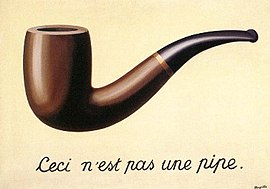
\includegraphics[width=0.9\textwidth]{pics/MagrittePipe.jpg}
			\caption{\url{https://en.wikipedia.org/wiki/The_Treachery_of_Images}}
		\end{figure}
	\end{columns}
\end{frame}

\begin{frame}
	\frametitle{``dplyr'': Grammar of Data Manipulation}
	\begin{columns}[onlytextwidth]
		\column{0.3\textwidth}
		\hspace*{0.5cm}
\includegraphics[width=0.4\textwidth]{../figs/dplyr.png}
		\begin{block}{Core ``verbs''}
			\begin{itemize}
				\item \ttfamily{select()}
				\item \ttfamily{filter()}
				\item \ttfamily{arrange()}
				\item \ttfamily{mutate()}
				\item \ttfamily{summarize()}
			\end{itemize}
		\end{block}
		
		\column{0.7\textwidth}
		\begin{block}{Dream team with pipe}
			\begin{itemize}
				\item Verbs take as first argument a dataframe and return modified dataframe
				\item On CRAN since 2014 (Hadley Wickham)
				\item Like ``magrittr'', part of tidyverse
				\item Translate between base R and dplyr?
			\end{itemize}
		\end{block}

		\begin{example}
		\end{example}
	\end{columns}
\end{frame}

\begin{frame}
	\frametitle{``ggplot2'': Grammar of Graphics}
	\begin{columns}
		\column{0.5\textwidth}
		\centering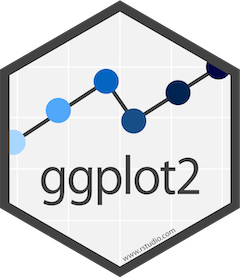
\includegraphics[width=0.3\textwidth]{../figs/ggplot2.png}
	
		\begin{block}{Modify plot layer per layer}
			\begin{itemize}
				\item Simple ``{\ttfamily +}'' instead of {\ttfamily \%>\%}
				\item On CRAN since 2007 
				
				(Hadley Wickham)
				\item Also in tidyverse
			\end{itemize}
		\end{block}
	
		\column{0.5\textwidth}
		\begin{block}{``plotly'' package}
			\begin{itemize}
				\item Interactive figures
				\item Wraps JavaScript library
				\item Can translate ggplot to Plotly
			\end{itemize}
		\end{block}
	
		\begin{example}
		\end{example}
	\end{columns}
	
\end{frame}

\begin{frame}
	\frametitle{Reports with R Markdown}
	\begin{columns}
		\column{0.4\textwidth}
		\hspace{1cm}
\includegraphics[width=0.3\textwidth]{../figs/rmarkdown.png}
		\begin{block}{Markdown text + R code}
			$\rightarrow$ HTML, Word, PDF
			
			On CRAN since 2014 (Yihui Xie)		
		\end{block}			
		
		\begin{example}
			\begin{itemize}
				\item Markdown syntax
				\item Simple R Markdown file
			\end{itemize}
		\end{example}
		
		\column{0.6\textwidth}
		\begin{block}{Workflow}
			\begin{enumerate}
				\item Create .Rmd with YAML header
				\item Write analysis and adapt YAML
				\item Hit ``Knit''/\texttt{rmarkdown::render()}
			\end{enumerate}
		\end{block}
	
		\begin{block}{When you hit ``Knit''}
			\begin{enumerate}
				\item \texttt{knitr::knit()} searchs code chunks, runs them and ``knits'' the results with your Markdown text to a temporary .md file
				\item The .md file is converted to desired output with Pandoc, using YAML header to specify its call 
			\end{enumerate}
		\end{block}
	
	\end{columns}
\end{frame}

%=====================================================================
\subsection{Writing Functions}
%=====================================================================

\begin{frame}
	\frametitle{Writing Functions}
	\begin{columns}
		\column{0.5\textwidth}
		\begin{block}{Already used many functions}
			\begin{itemize}
				\item \texttt{mean()}
				\item \texttt{ggplot2::ggplot()}
				\item \texttt{+}
			\end{itemize}
		\end{block}
	
		\begin{block}{Write \alert{own} functions to}
			\begin{itemize}
				\item avoid code duplication
				\item produce readable code
			\end{itemize}
			\begin{example}
			\end{example}
		\end{block}
	
		\column{0.5\textwidth}
		\begin{block}{Code style}
			\begin{itemize}
				\item Line length, curly braces, spaces?
				\item Comments: Why, not what
				\item Defensive programming: \texttt{if} + \texttt{stop()}
			\end{itemize}
		
			\begin{example}
			\end{example}
		\end{block}
		
		\begin{block}{Organizing functions}
			\texttt{source(functions.R)} or \alert{own package}
			\begin{example}
			\end{example}
		\end{block}
	\end{columns}
\end{frame}

\begin{frame}
	\frametitle{dplyr and ggplot2 in functions}

	\begin{block}{Unquoted variable names look nice}
		\begin{itemize}
			\item \texttt{diamonds \%>\% select(price, color)}
			\item \texttt{ggplot(diamonds, aes(x = color))}
			\item \texttt{facet\_grid($\sim$ color)}
		\end{itemize}
	\end{block}
	
	But what if ``price'' and/or ``color'' should be passed as function arguments?
	
	\vfill
	
	\begin{block}{Some solutions}
		\begin{itemize}
			\item \texttt{select(all\_of(c("price", "color")))} $\rightarrow$ \texttt{select(price, color)}
			\item \texttt{aes(x = .data[["color"]])} $\rightarrow$ \texttt{aes(x = color)}
			\item \texttt{reformulate("color")} $\rightarrow$ \texttt{$\sim$ color}
		\end{itemize}
	\end{block}

	\vfill
	
	\begin{example}
	\end{example}
\end{frame}

\begin{frame}
	\frametitle{plot, print, summary}
	\begin{block}{Generic functions}
		\begin{itemize}
			\item plot, print, summary, predict, \dots
			\item Depend on \alert{class} of object
		\end{itemize}
	
		\begin{example}
		\end{example}
	\end{block}

	\begin{block}{S3 System}
		\begin{itemize}
			\item Simple object oriented system
			\item Generic function calls \texttt{UseMethod()} to find class method, e.g.
		 
		 		\texttt{plot()} $\rightarrow$ \texttt{UseMethod()} $\rightarrow$ \texttt{plot.factor()}
			\item Write new class method of existing generic function
			\item Or write new generic
		\end{itemize}
	
		\begin{example}
		\end{example}
	\end{block}
\end{frame}
%%=====================================================================
\section{Statistical Inference}
%=====================================================================

\begin{frame}
	\frametitle{Outline}
	
	\begin{enumerate}
		\item Statistical Inference
		\item The Bootstrap
		\item Permutation Tests
	\end{enumerate}
	
	\vfill
	
	\begin{block}{Aims}
		\begin{itemize}
			\item Learn computer-intensive methods in statistical inference
			\item Apply programming techniques from last chapter
		\end{itemize}
	\end{block}
\end{frame}

%=====================================================================
\subsection{Statistical Inference}
%=====================================================================

\begin{frame}
	\frametitle{Statistical Inference}
	Use data to make statements about unknown population parameter $\theta$:
	\begin{itemize}
		\item True proportion of patients that benefit from some novel treatment
		\item True average claim count per insured car year
		\item True correlation coefficient between the price of a diamond and its size
	\end{itemize}
	
	\vfill
	
	\begin{block}{Main Tasks}
		\begin{enumerate}
			\item Point estimation: Estimate $\theta$ by an estimator $\hat \theta(\text{data})$
			\item Interval estimation: Provide confidence interval $I(\text{data})$ for $\theta$
			\item Testing: Use test statistic $T(\text{data})$ to measure statistical evidence against null hypothesis like $\theta_o = 0$. Reject if evidence is strong enough
		\end{enumerate}
	\end{block}
	
	Math stats solves tasks for different parameters $\theta$, and under different circumstances
\end{frame}

\begin{frame}
	\frametitle{Classic Results for the Mean}
	\begin{itemize}
		\item Distribution $F$ with $\mu = \E(F)$ and $\sigma = \sqrt{\text{Var}(F)} < \infty$
		\item Sample $\boldsymbol X = (X_1, \dots, X_n)$ of independent random variables drawn from $F$
	\end{itemize}
	
	\vfill
	
	\begin{block}{What can we say about the sample mean $\hat \mu = \frac{1}{n}\sum_{i = 1}^n X_i$ as an estimator of $\mu$?}
		\begin{enumerate}
			\item $\hat \mu$ is unbiased: 
			$$
			  \E(\hat \mu) = \E\left(\frac{1}{n}\sum_{i = 1}^n X_i\right) = \frac{1}{n}\sum_{i = 1}^n \E(X_i) = \mu
			$$
			\item Law of large numbers: As $n\to \infty$, $\hat\mu$ converges in probability to $\mu$
			\item CLT: For $Z\sim N(0, 1)$ and standard deviation $\sigma(\hat\mu)$ of $\hat\mu$:
			$$
			  \frac{\hat\mu - \mu}{\sigma(\hat\mu)} \xrightarrow[n\to \infty]{d} Z
			$$
		\end{enumerate}
	\end{block}
\end{frame}

\begin{frame}
	\frametitle{Standard Deviation $\sigma(\hat\mu)$ of the Sample Mean}
	$$
	  \sigma(\hat\mu) = \sqrt{\text{Var}(\hat\mu)} = \sqrt{\text{Var}\left(\frac{1}{n} \sum_{i = 1}^n X_i\right)} = \sqrt{\frac{1}{n^2} \sum_{i = 1}^n \text{Var}(X_i)} = \sqrt{\frac{1}{n} \text{Var}(X_i)} = \frac{\sigma}{\sqrt{n}}
	$$
	
	\vfill
	
	Since $\sigma = \sigma(F) = \sigma(X_i)$ unknown, replace it by \alert{sample} standard deviation
	$
	  \hat\sigma = \sqrt{\frac{1}{n-1}\sum_{i = 1}^{n}(X_i - \hat\mu)^2}
	$
	$\rightarrow$ estimated standard deviation of mean: $\hat\sigma(\hat\mu) = \hat\sigma / \sqrt{n}$
	
	\vfill
	
	\begin{block}{Remarks and outlook}
		\begin{itemize}
			\item Standard deviation $\sigma(\hat\theta)$ of estimator called \alert{standard error}
			\item \alert{Estimated} standard error denoted by $\hat\sigma(\hat\theta)$
			\item Accuracy of estimator $\rightarrow$ confidence intervals for $\theta$
			\item Formulas are rare $\rightarrow$ Bootstrap
		\end{itemize}
	\end{block}
\end{frame}

\begin{frame}
	\frametitle{Computer Simulations}
	\begin{exampleblock}{Illustrations via repeated sampling from known(!) distribution}
		\begin{itemize}
			\item Law of large numbers
			\item Central Limit Theorem
		\end{itemize}
	\end{exampleblock}
\end{frame}

\begin{frame}
	\frametitle{From the CLT to Confidence Intervals (CI)}
	Approximate $(1-\alpha)\cdot 100\%$-CI for $\mu$:
	$$
	  [\hat\mu \pm z_{1-\alpha/2} \hat\sigma(\hat\mu)],
	$$
	where $\hat\sigma(\hat\mu) = \hat\sigma / \sqrt{n}$, and $z_\beta$ is the $\beta$-quantile of $N(0,1)$ ($\rightarrow$ lecture notes)
	
	\vfill
	
	\begin{block}{Remarks}
		\begin{itemize}
		\item ``z-confidence interval'' for the mean $\mu$
		\item Usually more accurate: Student CI with $n-1$ degrees of freedom
		\item ``Probability'' or ``Confidence''?
		\end{itemize}
	\end{block}
	
	\begin{exampleblock}{Examples}
		\begin{itemize}
			\item z-CI for the mean
			\item Accuracy: Compare nominal coverage probability $1-\alpha$ and real coverage
		\end{itemize}
	\end{exampleblock}
\end{frame}

\begin{frame}
	\frametitle{Other Estimators}
	\begin{itemize}
		\item Many estimators $\hat \theta$ are asymptotically normal
		\item We can use the same formula to calculate approximate $(1-\alpha)\cdot 100\%$ CI for $\theta$:
			$$
		 		I_{1-\alpha} = [\hat \theta \pm z_{1-\alpha/2} \hat \sigma(\hat\theta)]
			$$
	\end{itemize}
	
	\vfill
	
	\begin{block}{Limitation}
		Usually, no general formula for $\hat \sigma(\hat\theta)$ available
	\end{block}
	
	\begin{block}{Solution (Bradley Efron, 1979)}
		\alert{The Bootstrap} offers a fully generic and automatic way of finding $\hat \sigma(\hat\theta)$
	\end{block}	
\end{frame}

%=====================================================================
\subsection{The Bootstrap}
%=====================================================================

\begin{frame}
	\frametitle{The Bootstrap}
	\begin{itemize}
		\item Observe sample: $\bx = (x_1, \dots, x_n)$
		\item Standard error $\hat \sigma(\hat\theta)$ of estimator $\hat\theta(\bx)$? 
	\end{itemize}
	
	\begin{block}{Bootstrap estimate of standard error}
		\begin{enumerate}
			\item From $\bx$, draw with replacement a \alert{Bootstrap sample} $\bx^*$ of size $n$ 
			\item Calculate \alert{Bootstrap replication} $\hat \theta(\bx^*)$ of $\hat\theta(\bx)$
			\item Repeat $B$ times to get $B$ Bootstrap replications $\hat \theta(\bx^{*1}), \dots, \hat \theta(\bx^{*B})$
			\item Calculate \alert{sample standard deviation} of the $B$ replications
		\end{enumerate}
	\end{block}
	
	\begin{columns}[onlytextwidth]
		\column{0.33\textwidth}
		\begin{exampleblock}{Examples}
		\begin{itemize}
			\item Mean
			\item Median
		\end{itemize}
		\end{exampleblock}

	\column{0.67\textwidth}
	\begin{itemize}
		\item Why ``Bootstrap''?
		\item Bootstrap sample is to original sample what 
		
		original sample is to population
	\end{itemize}
	\end{columns}
\end{frame}


\begin{frame}
	\frametitle{Bootstrap Confidence Intervals}
	\begin{block}{Standard normal Bootstrap confidence interval}
		\begin{itemize}
			\item Take any asymptotically normal $\hat \theta$
			\item Approximate $(1-\alpha)\cdot 100\%$-confidence interval for $\theta$:
				$$
		 			[\hat \theta \pm z_{1-\alpha/2} \hat \sigma(\hat\theta)]
				$$
			\item $\hat \sigma(\hat\theta)$: Bootstrap estimate of standard error
			\item Sample size not too small
		\end{itemize}
	\end{block}
	
	\vfill
	
	\begin{example}
	\end{example}
\end{frame}

\begin{frame}
	\frametitle{Alternative: Percentile Bootstrap Confidence Interval}
	\begin{itemize}
		\item Consider $B$ Bootstrap replications $\hat \theta(\bx^{*1}), \dots, \hat \theta(\bx^{*B})$
		\item Use empirical $(\alpha/2)$ and $(1-\alpha/2)$ quantiles as confidence limits
		\item No asymptotic normality of $\hat\theta$ required
		\item Transformation respecting
		\item Range-preserving
		\item Since extreme quantiles involved, use large $B$, e.g., 9999
	\end{itemize}
	
	\begin{exampleblock}{Examples}
	\begin{itemize}
		\item Median
		\item Simulation study on accuracy
		\item Better confidence intervals
	\end{itemize}
	\end{exampleblock}
\end{frame}

\begin{frame}
	\frametitle{Multiple Samples/Groups}
	\begin{block}{Examples}
		\begin{itemize}
			\item Mean difference between two groups
			\item Median difference between two groups
			\item R-squared of a one-way ANOVA between multiple groups
		\end{itemize}
	\end{block}

	\vfill
	
	\begin{block}{Two ways of drawing Bootstrap sample}
		\begin{enumerate}
			\item Resampling within group to keep group sizes fixed (usually recommended)
			\item Resample rows in data with one column representing the group (more generic)
		\end{enumerate}
	\end{block}

	\vfill
	
	\begin{example}
	\end{example}

\end{frame}

\begin{frame}
	\frametitle{Multivariate Estimators}
	\begin{block}{Examples}
		\begin{itemize}
			\item Pearson correlation
			\item Kendall's rank correlation
			\item R-squared of a linear regression
			\item Mean difference of two groups (how?)
		\end{itemize}
		$\rightarrow$ Study associations between variables
	\end{block}
	
	\vfill
	
	\begin{block}{How to create Bootstrap sample?}
		Sample whole \alert{rows} of dataset (with replacement)
	\end{block}

	\vfill
	
	\begin{example}
	\end{example}

\end{frame}

\begin{frame}
	\frametitle{Permutation Tests}
	First described by R.A. Fisher in 1935!
	
	\vfill
	
	\begin{block}{Hypotheses tests in general}
		\begin{itemize}
			\item Want to show interesting alternative hypothesis $H_1$ about $\theta$, e.g. $\theta \ne 0$
			\item Measure evidence against contrary $H_0$, e.g. $\theta = 0$ by test statistic $T$
			\item If evidence is strong enough, reject $H_0$ in favor of $H_1$
		\end{itemize}
	\end{block}
	
	\begin{block}{p value}
		Probability of observing at least as much evidence against $H_0$ as in the specific sample when $H_0$ holds $\rightarrow$ reject $H_0$ if p value $\le 0.05$ (or some other prespecified value)
		$$
			\text{p value} = P_{H_0}\{T \ge t\}
		$$
	\end{block}
	
	\begin{example}
	\end{example}
\end{frame}

\begin{frame}
	\frametitle{Tests for Association}
	
	Example showed: two-sample t test is test of association between:
	\begin{itemize}
		\item $\boldsymbol Y$: Numeric variable representing the stacked values of \alert{both} groups
		\item $\bX$: Binary variable representing the group (``A'' or ``B'')
	\end{itemize}
	
	Association is measured in terms of location shift in the grouped means
	
	\vfill
	
	Many additional tests are tests of association between two variables. Examples?
	
	\vfill
	
	Can be tackled by 
	\begin{itemize}
		\item computer-intensive,
		\item fully automatic
	\end{itemize}
	technique called \alert{permutation test}
\end{frame}

\begin{frame}
	\frametitle{Permutation Tests}
	$T$: Measures strength of association between $\bX$ and $\boldsymbol Y$ with observations $\bx$ and $\boldsymbol y$
	
	\vfill
	
	\begin{block}{How to find distribution of $T$ under null?}
		\begin{enumerate}
			\item $\bx^*$: permutation of $\bx$
			
			$\rightarrow$ destroys dependency between $\bx$ and $\boldsymbol y$
			\item Calculate $t^* = T(\bx^*, \boldsymbol y)$
			\item Repeat above steps $B$ times to get permutation replications $t^*(1), \dots, t^*(B)$
			
			$\rightarrow$ empirical null hypothesis distribution of $T$
			\item Bootstrap p value: $\frac{1}{B}\sum_{i = 1}^B 1\{t^*(i) \ge T(\bx, \boldsymbol y)\}$
		\end{enumerate}
	\end{block}
\end{frame}

\begin{frame}
	\frametitle{Remarks and Examples}
	\begin{block}{Remarks}
		\begin{itemize}
			\item $B$ large, e.g. $10000$
			\item Why not all permutations? $\rightarrow$ Approximate or Monte-Carlo permutation tests
			\item ``coin'' package in R
			\item Permutation replications versus Bootstrap replications?
			\item Not completely assumption-free (iid.\ is sufficient)
		\end{itemize}
	\end{block}
	
	\begin{exampleblock}{Examples}
		\begin{itemize}
			\item Two-sample test
			\item Simulation: Type 1 error and power?
		\end{itemize}
	\end{exampleblock}
\end{frame}

\begin{frame}
	\frametitle{More Examples}
	
	\begin{itemize}
		\item Wilcoxon's rank sum test
		\item Test for Pearson correlation
		\item Paired t-test
	\end{itemize}
	
	\vfill
	
	Many more in the ``coin'' package
\end{frame}

%=====================================================================
\subsection{Permutation Tests}
%=====================================================================
%%=====================================================================
\section{Linear Models}
%=====================================================================

\begin{frame}
	\frametitle{Outline}
	
	\begin{itemize}
		\item Start of ``Statistical ML in Action''
		\item Linear Regression
		\item Generalized Linear Models (GLM)
		\item Modeling Large Data
	\end{itemize}
\end{frame}

%=====================================================================
\subsection{Statistical ML in Action}
%=====================================================================

\begin{frame}
	\frametitle{Statistical ML in Action}
	\begin{columns}
		\column{0.55\textwidth}
		\begin{block}{What is ML?}
			Collection of statistical algorithms used to
			\begin{enumerate}
				\item predict things (supervised ML) or to
				\item investigate data structure (unsupervised)
			\end{enumerate}
		\end{block}
		
		\begin{figure}
			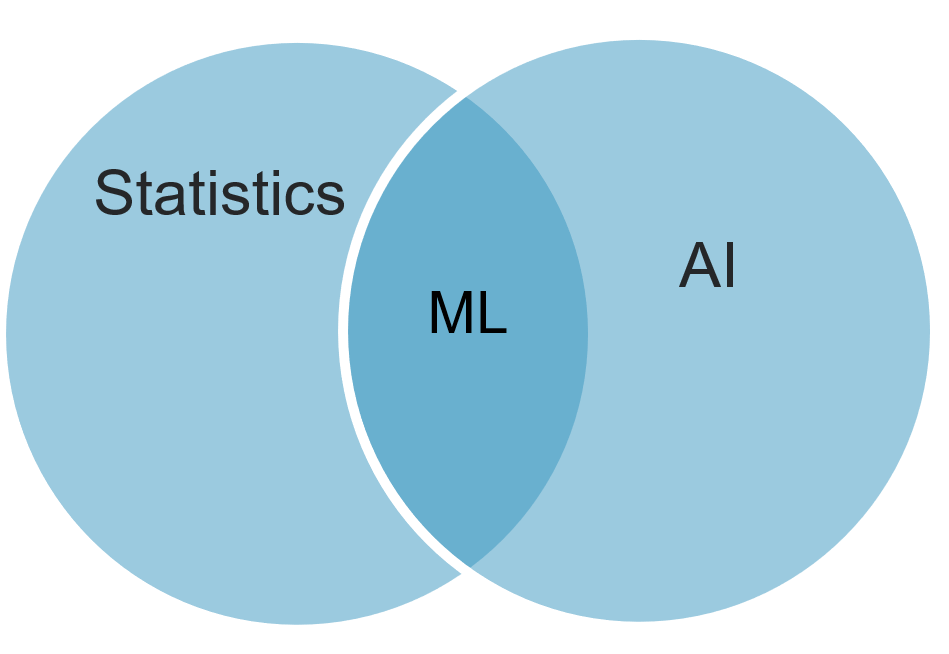
\includegraphics[width=0.6\textwidth]{pics/ml.png}
		\end{figure}
		
		\column{0.4\textwidth}
		\begin{block}{Focus on supervised ML}
			\begin{itemize}
				\item Regression
				\item Classification
			\end{itemize}
		\end{block}
		
		\begin{block}{Chapters}
			\begin{itemize}
				\item[3.] Linear Models
				\item[4.] Model Selection and Validation
				\item[5.] Trees
				\item[6.] Neural Nets
			\end{itemize}
		\end{block}
	\end{columns}
\end{frame}

\begin{frame}
	\frametitle{Model Setup}
	Approximate property $T$ of \alert{response} $Y$ (often $T = \E$) by function $f$ of $p$-dim \alert{covariate} vector $\bX = (X^{(1)}, \dots, X^{(p)})$ with value $\bx = (x^{(1)}, \dots, x^{(p)})$, i.e.,
	$$
		T(Y\mid \bX = \bx) \approx f(\bx)
	$$
	\vspace{-1.5em}
	\begin{itemize}
		\item Abbreviate $T(Y\mid \bX = \bx) = T(Y\mid \bx)$
		\item Estimate $f$ by $\hat f$ from data by minimizing objective
		$$
		Q(f) = \sum_{i = 1}^n L(y_i, f(\bx_i)) + \lambda \Omega(f)
		$$
		\item $L$: loss function in line with $T$; $\lambda \Omega(f)$: optional penalty
		\item $\boldsymbol y = (y_1, \dots, y_n)^T$: observed values of $Y$
		\item $\boldsymbol{\hat y} = (\hat y_1, \dots, \hat y_n)^T$: predicted/fitted values $\hat y_i = \hat f(\bx_i)$
		\item $\bx_1, \dots, \bx_n$: $n$ feature vectors; $x_i^{(j)}$: $i$-th value of $X^{(j)}$; $\bx^{(j)}$: $n$ values of feature $X^{(j)}$
	\end{itemize}
\end{frame}

%=====================================================================
\subsection{Linear Regression}
%=====================================================================

\begin{frame}
	\frametitle{Linear Regression}
	\begin{itemize}
		\item Postulate model equation
		$$
		\E(Y \mid \bx) = f(\bx) = \beta_o + \beta_1 x^{(1)} + \dots + \beta_p x^{(p)}
		$$
		\item Interpretation of parameters $\beta_j$? Ceteris Paribus!
		\item Optimal $\hat \beta_j$? Minimize sum of squared errors/residuals
		$$
		\sum_{i = 1}^n (\underbrace{y_i - \hat y_i}_{\text{\alert{Residual}}})^2 
		$$
		\item Remember: $\hat y = \hat f(\bx)$ are \alert{predictions}
	\end{itemize}
	
	\vfill
	
	\begin{example}
		Simple linear regression: $\E(Y \mid x) = \alpha + \beta x$
	\end{example}
\end{frame}

\begin{frame}
	\frametitle{Aspects of Model Quality}
	\begin{columns}[onlytextwidth]
		\column{0.5\textwidth}
		\begin{block}{Predictive performance}
			\begin{itemize}
				\item $\text{\alert{MSE}} = \frac{1}{n}\sum_{i = 1}^n (y_i - \hat y_i)^2$
				\item Root-MSE (\alert{RMSE})
				\item Relative performance: $R^2 = 1 - \text{MSE}/\text{MSE}_0$
				\item $\text{MSE}_0 \rightarrow$ intercept-only model
			\end{itemize}
		\end{block}	
		
		\column{0.5\textwidth}
		\begin{block}{Validity of assumptions}
			\begin{itemize}
				\item Model equation is correct
				\item \alert{Normal} linear model
				$$
				Y = f(\bx) + \varepsilon \text{ with }
				\varepsilon \sim N(0, \sigma^2)
				$$
			\end{itemize}
		\end{block}
	\end{columns}
	
	\vfill
	
	\begin{exampleblock}{\centering Example}
	\end{exampleblock}
\end{frame}

\begin{frame}
	\frametitle{Typical Problems}
	\begin{figure}
		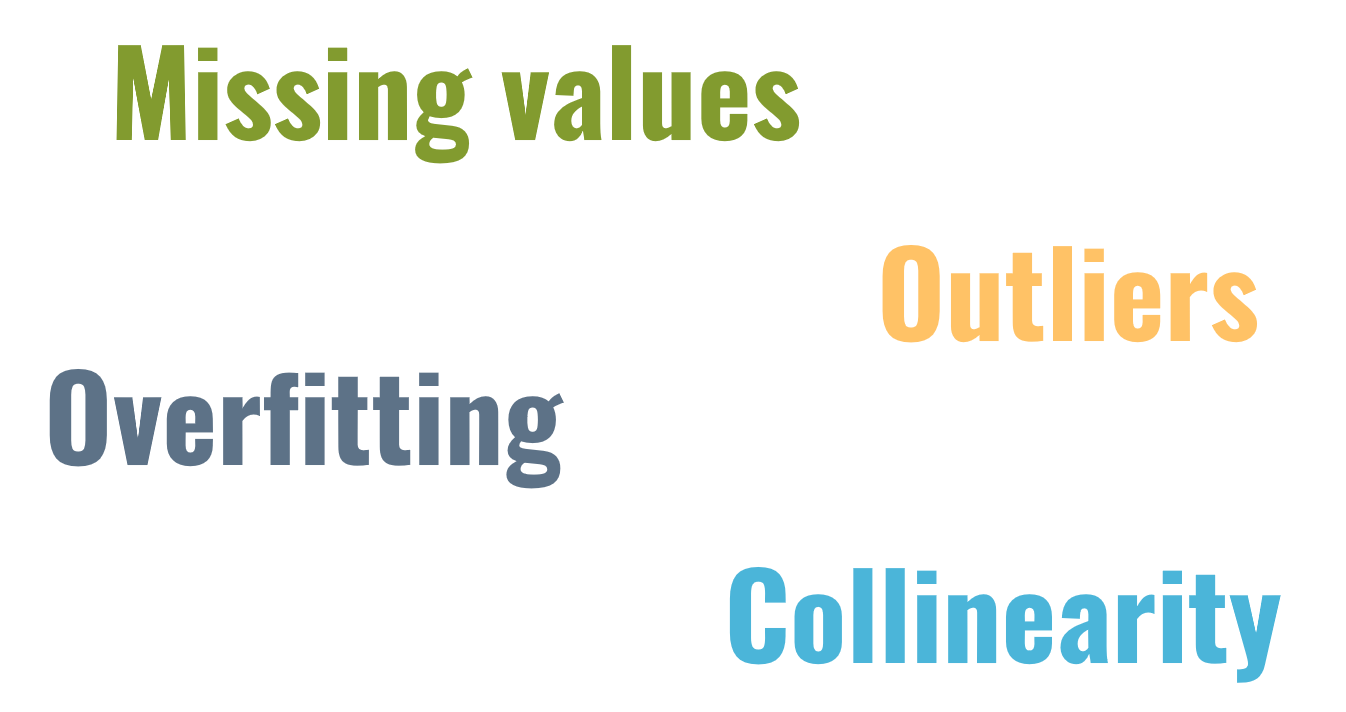
\includegraphics[width=0.7\textwidth]{pics/linear_problems.png}
	\end{figure}
\end{frame}

\begin{frame}
	\frametitle{Categorical Covariates}
	\begin{columns}[onlytextwidth]
		\column{0.45\textwidth}
		\begin{itemize}
			\item One-Hot-Encoding
			\item Dummy coding
			\item Interpretation?
		\end{itemize}
		
		\vspace{1cm}
		
		\begin{example}
		\end{example}
		
		\column{0.45\textwidth}
		\begin{block}{\centering Example of One-Hot-Encoding}
			\begin{small}
				\begin{table}
					\begin{tabular}{c|ccccccc}
						color& D& E& F &G&H &I &J \\
						\hline
						E  &   0  &   1  &   0  &   0  &   0  &   0  &   0 \\
						E  &   0  &   1  &   0  &   0  &   0  &   0  &   0 \\
						E  &   0  &   1  &   0  &   0  &   0  &   0  &   0 \\
						I  &   0  &   0  &   0  &   0  &   0  &   1  &   0 \\
						J  &   0  &   0  &   0  &   0  &   0  &   0  &   1 \\
						J  &   0  &   0  &   0  &   0  &   0  &   0  &   1 \\
						I  &   0  &   0  &   0  &   0  &   0  &   1  &   0 \\
						H  &   0  &   0  &   0  &   0  &   1  &   0  &   0 \\
						E  &   0  &   1  &   0  &   0  &   0  &   0  &   0 \\
						H  &   0  &   0  &   0  &   0  &   1  &   0  &   0 \\
						\hline
					\end{tabular}
				\end{table}
			\end{small}
		\end{block}
	\end{columns}
\end{frame}

\begin{frame}
	\frametitle{Linear Regression is Flexible}
	\begin{enumerate}
		\item Non-linear terms
		\item Interactions
		\item Transformations like logarithms
	\end{enumerate}
	
	\vfill
	
	\begin{alertblock}{These elements are essential but tricky!}
	\end{alertblock}
\end{frame}

\begin{frame}
	\frametitle{Non-Linear Terms}
	\begin{columns}
		\column{0.5\textwidth}
		\begin{block}{Deal with non-linear associations to $Y$?} $\rightarrow$ invest more parameters
			\begin{enumerate}
				\item Polynomial terms
				\begin{itemize}
					\item E.g., cubic regression
					$$
					\E(Y \mid x) = \beta_0 + \beta_1 x + \beta_2 x^2 + \beta_3 x^3
					$$
					\item Don't extrapolate!
				\end{itemize}
				\item Regression splines
			\end{enumerate}
		\end{block}
		
		\column{0.5\textwidth}
		\begin{block}{\centering Cubic terms for carat}
			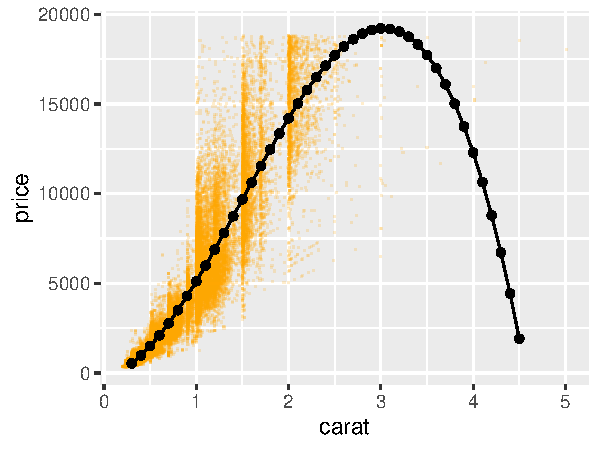
\includegraphics[width=1\textwidth]{pics/nonlinear.pdf}
			\vspace{-9em}
			\begin{scriptsize}
				\begin{table}
					\raggedleft
					\begin{tabular}{ccc}
						carat & carat$^2$ & carat$^3$ \\
						\hline
						0.23       &            0.0529       &          0.012167\\
						0.21       &            0.0441       &          0.009261\\
						0.23       &            0.0529       &          0.012167\\
						\hline
					\end{tabular}
				\end{table}
			\end{scriptsize}
			\vspace{3em}
			\centering Use systematic predictions
		\end{block}
	\end{columns}
\end{frame}

\begin{frame}
	\frametitle{Interactions}
	\begin{columns}
		\column{0.55\textwidth}
		\begin{itemize}
			\item Additivity of effects not always realistic
			$$
			\E(Y \mid \bx) = \beta_o + \beta_1 x^{(1)} + \dots + \beta_p x^{(p)}
			$$
			\item Adding interaction terms brings necessary flexibility 
			$\rightarrow$ more parameters
			\item Interaction between features $X$ and $Z$
			\begin{itemize}
				\item Multiplication (for categoricals?)
				\item For categorical $Z$, effects of $X$ are calculated by level of $Z$
				\item Like separate models per level of $Z$
			\end{itemize}
		\end{itemize}
		
		\column{0.45\textwidth}
		\begin{block}{\centering Carat and color}
			\begin{figure}
				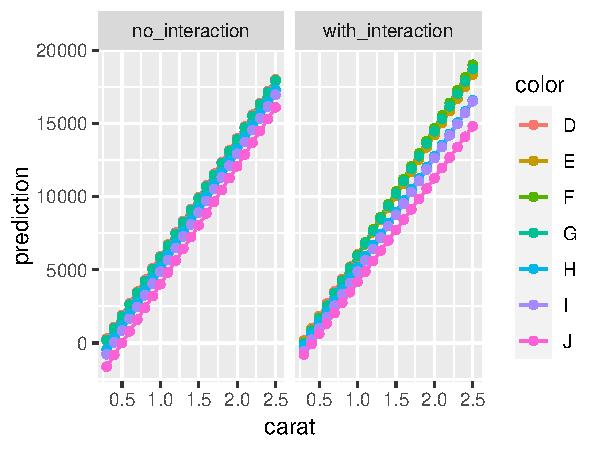
\includegraphics[width=\textwidth]{pics/interaction.pdf}
			\end{figure}
		\end{block}
	\end{columns}
\end{frame}

\begin{frame}
	\frametitle{Transformations of Covariates}
	\begin{block}{Examples}
		\begin{itemize}
			\item Dummy variables for categoricals
			\item Decorrelation
			\item Logarithms against outliers
		\end{itemize}
	\end{block}
	
	\vfill
	
	Effects are interpreted for transformed covariates
\end{frame}

\begin{frame}
	\frametitle{Logarithmic Covariates}
	\begin{itemize}
		\item $\E(Y \mid x) = \alpha + \beta\log(x)$
		\item Properties of logarithm allow interpretation \alert{for original covariate}
		\item A 1\% increase in $X$ is associated with an increase in $\E(Y)$ of about $\beta/100$
		\item Why?
		\begin{align*}
			\E(Y\mid 1.01x) - \E(Y\mid x) &= \alpha + \beta \log (1.01x) - \alpha - \beta \log(x) \\
			&= \beta \log\left(\frac{1.01x}{x}\right) \\
			&= \beta \log(1.01) \approx \beta/100
		\end{align*}
	
		\vfill
		
		\begin{example}
		\end{example}
	\end{itemize}
\end{frame}

\begin{frame}
	\frametitle{Logarithmic Responses}
	We see: log-transforming $X$ allows to talk about relative effects in $X$
	
	\vfill
	
	\begin{block}{Idea: log-transformed $Y$ allows to talk about relative effects on $Y$}
		Assume for a moment that
		$$
			\E(\log(Y) \mid x) = \alpha + \beta x \implies \log(\E(Y \mid x)) = \alpha + \beta x
		$$
		\vspace*{-1.2em}
		\begin{itemize}
			\item Multiplicative model $\E(Y\mid x) = e^{\alpha + \beta x}$
			\item Relative interpretation: ``A one-point increase in $X$ is associated with a relative increase in $\E(Y)$ of $100\%(e^\beta - 1)\approx 100\% \beta$''
			\item If also $\log(X)$?
		\end{itemize}
	\end{block}

	\vfill
	
	But assumption is wrong $\rightarrow$ biased predictions for $Y$ $\rightarrow$ GLMs

	\vfill
	
	\begin{exampleblock}{Examples}
	\end{exampleblock}
\end{frame}

\begin{frame}
	\frametitle{Example: Realistic Model for Diamond Prices}
	\begin{columns}
		\column{0.55\textwidth}
		\begin{itemize}
			\item Response: log(price)
			\item Covariates: log(carat), color, cut and clarity
		\end{itemize}
		
		\column{0.35\textwidth}
		\begin{figure}
			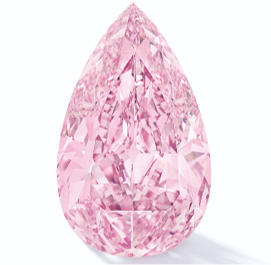
\includegraphics[width=0.7\textwidth]{pics/dia2.png}
		\end{figure}
	\end{columns}
\end{frame}

%=====================================================================
\subsection{Generalized Linear Models}
%=====================================================================

\begin{frame}
	\frametitle{Generalized Linear Model (GLM)}
	\begin{block}{(One) extension of linear regression}
	\end{block}
	
	\begin{block}{Model equation}
		Two equivalent formulations
		\begin{align*}
			g(\E(Y \mid \bx)) &= \eta(\bx) = \beta_o + \beta_1 x^{(1)} + \dots + \beta_p x^{(p)} \\
			\E(Y \mid \bx) &=g^{-1}(\eta(\bx)) =  g^{-1}(\beta_o + \beta_1 x^{(1)} + \dots + \beta_p x^{(p)})
		\end{align*}
	\end{block}
	
	\begin{block}{Components}
		\begin{itemize}
			\item Linear function/predictor $\eta$
			\item Link function $g$ to map $\E(Y \mid \bx)$ to linear scale
			\item Distribution of $Y$ conditional on covariates $\rightarrow$ loss function (unit deviance)
		\end{itemize}
	\end{block}
\end{frame}

\begin{frame}
	\frametitle{Typical GLMs}
	\begin{columns}[onlytextwidth]
		\column{0.75\textwidth}
		\begin{figure}
			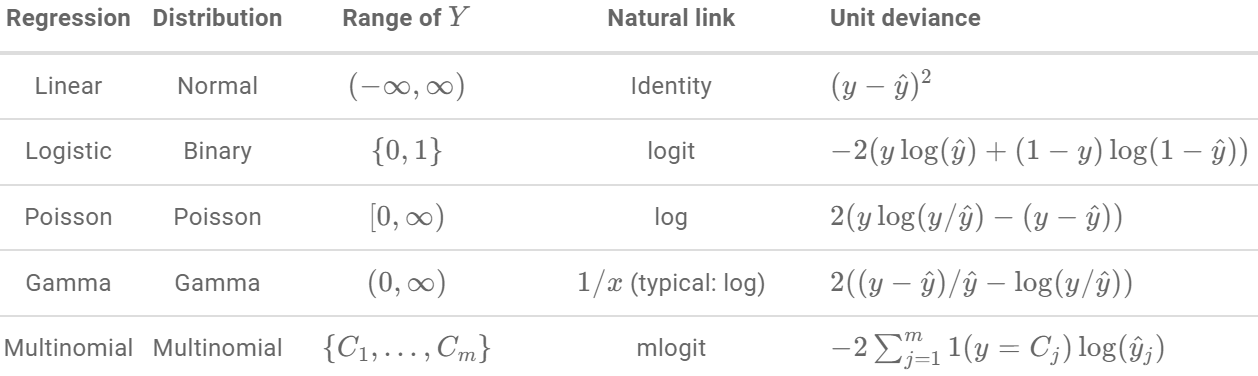
\includegraphics[width=1\textwidth]{pics/glm.png}
		\end{figure}
		\begin{figure}
			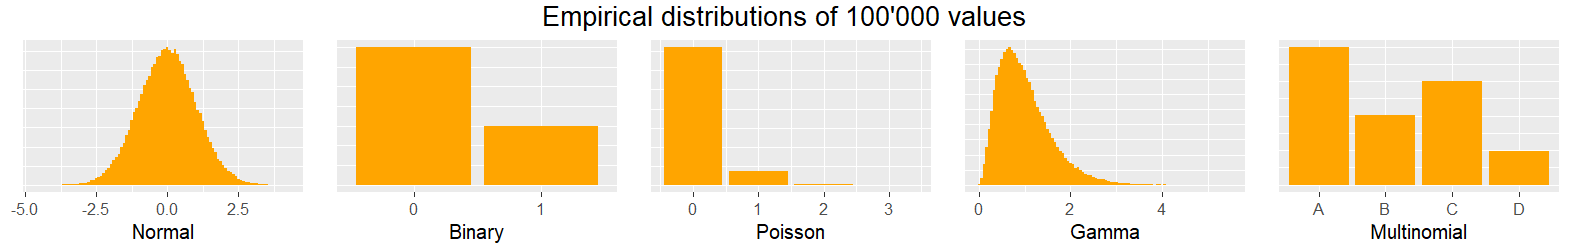
\includegraphics[width=1\textwidth]{pics/GLM_distributions.pdf}
		\end{figure}
		\column{0.25\textwidth}
		\begin{footnotesize}
			\begin{itemize}
				\itemsep0em 
				\item Predictions?
				\item Log-Link?
				\item For binary $Y$:
				$\E(Y) = P(Y = 1) = p$
				\item MSE $\rightarrow$ Deviance
				\item Losses in ML?
			\end{itemize}
		\end{footnotesize}
	\end{columns}
\end{frame}

\begin{frame}
	\frametitle{Why GLM, not Linear Regression?}
	\begin{block}{Linearity assumption not always realistic}
		\begin{enumerate}
			\item Binary $Y$: 
			
			Jump from 0.5 to 0.6 success probability less impressive than from 0.89 to 0.99
			\item Count $Y$: Jump from $\E(Y)$ of 2 to 3 less impressive than from 0.1 to 1.1.
			\item Right-skewed $Y$: 
			
			Jump from 1 Mio to 1.1 Mio deemed larger than from 2 Mio to 2.1 Mio.
		\end{enumerate}
		\alert{Logarithmic $Y$ not possible in the first two cases}
	\end{block}
	
	\vfill
	
	\begin{block}{GLM solves problem by suitable link $g$}
	\end{block}
	
	\vfill
	
	\begin{block}{Further advantages?}
	\end{block}
\end{frame}

\begin{frame}
	\frametitle{Interpretation of Effects guided by Link}
	\begin{columns}[onlytextwidth]
		\column{0.5\textwidth}
		\begin{block}{Identity link}
			Like linear regression
		\end{block}
		
		\begin{block}{Log link}
			Like linear regression with log response
			\begin{itemize}
				\item Multiplicative model for response
				\item Now in mathematically sound way
			\end{itemize}
		\end{block}
		
		\column{0.5\textwidth}
		\begin{block}{Logit link}
			\begin{itemize}
				\item Additive model for $\text{logit}(p)$
				\item $\text{logit}(p) = \text{\alert{log}}(\text{odds}(p)) = \text{\alert{log}}\left(\frac{p}{1-p}\right)$
				\item Remember: $p = P(Y=1) = \E(Y)$				
				\item Multiplicative model for $\text{odds}(p)$
				\item Coefficients \alert{$e^\beta - 1 \approx 100\%\beta$} interpreted as odds ratios
			\end{itemize}
		\end{block}
	\end{columns}
\end{frame}

\begin{frame}
	\frametitle{Examples with Insurance Claim Data}
	\begin{enumerate}
		\item Poisson regression for claim counts
		\item Binary logistic regression for claim (yes/no)
	\end{enumerate}
\end{frame}

%=====================================================================
\subsection{Modeling Large Data}
%=====================================================================

\begin{frame}
	\frametitle{Modeling Large Data}
	\begin{columns}[onlytextwidth]
		\column{0.55\textwidth}
		\begin{block}{As per 2023}
			\begin{itemize}
				\item On normal laptops, we can model datasets up to 8 GB in size
				(1 Mio iris data)
				\item Cloud computing allows 1000 times more
				\item We focus on in-memory situations
				
				$\rightarrow$ data fits in RAM
			\end{itemize}
		\end{block}
		
		\column{0.45\textwidth}
		\begin{block}{Aspect and example technology}
			\begin{enumerate}
				\item Data storage $\rightarrow$ Apache Parquet
				\item Data loading $\rightarrow$ Apache Arrow
				\item Preprocessing $\rightarrow$ data.table
				\item Modeling $\rightarrow$ H2O
			\end{enumerate}
			\vphantom{a}
		\end{block}
	\end{columns}

	\vfill
	
	\begin{example}
	\end{example}
\end{frame}

%%=====================================================================
\section{Model Selection and Validation}
%=====================================================================

\begin{frame}
	\frametitle{Two Questions}
	
	\begin{itemize}
		\item ``How good is our model?''
		\item ``Which model to choose among alternatives?''
	\end{itemize}
	
	\vfill
	
	\begin{columns}[onlytextwidth]
		\column{0.45\textwidth}
		\begin{block}{Problem and solution}
			\begin{itemize}
				\item ``In-sample'' performance is biased
				\item Overfitting should not be rewarded
				\item Use data splitting to get fair results
			\end{itemize}
		\end{block}
		
		\column{0.55\textwidth}
		\begin{alertblock}{Notation}
			\begin{itemize}
				\item Total loss $Q(f, D) = \sum_{(y_i, \bx_i) \in D} L(y_i, f(\bx_i))$
				\item Average loss $\bar Q(f, D) = Q(f, D) / |D|$
				\item Performance measure or evaluation metric $S(f, D)$ of interest, often $S = \bar Q$ or a function of it
			\end{itemize}
		\end{alertblock}
	\end{columns}
\end{frame}

\begin{frame}
	\frametitle{Outline}
	\begin{itemize}
		\item Nearest-Neighbor
		\item Simple Validation 
		\item Cross-Validation
		\item Test Data and Final Workflow
		\item Excursion: SQL and Spark
	\end{itemize}
\end{frame}

%=====================================================================
\subsection{Nearest-Neighbor}
%=====================================================================

\begin{frame}
	\frametitle{Excursion: $k$-Nearest-Neighbor ($k$-NN)}
	\begin{itemize}
		\item Alternative to linear model
		\item How does it work?
		\item Classification and regression
		\item Standardization?
	\end{itemize}
	
	\vfill
	
	\begin{example}
	\end{example}
\end{frame}

%=====================================================================
\subsection{Simple Validation}
%=====================================================================

\begin{frame}
	\frametitle{Simple Validation}
	\begin{itemize}
		\item In-sample, 1-NN would win any comparison!?
		\item Split data into training and validation sets $D_\text{train}$ and $D_\text{valid}$, e.g., 80\%/20\%
		\item Use performance $S(\hat f, D_\text{valid})$ on validation set to make decisions 
		
		(choose models, choose parameters like $k$)
		\item Measure amount of overfitting/optimism by 
		$$
		S(\hat f, D_\text{valid}) - S(\hat f, D_\text{train})
		$$
	\end{itemize}
	
	\vfill
	
	\begin{example}
	\end{example}
\end{frame}

%=====================================================================
\subsection{Cross-Validation}
%=====================================================================

\begin{frame}
	\frametitle{$K$-fold Cross-Validation (CV)}
	Simple validation is neither economic nor robust, except for large data
	
	\vfill
	
	\begin{columns}[onlytextwidth]
		\column{0.65\textwidth}
		\begin{block}{Algorithm}
			\begin{enumerate}
				\item Split the data into $K$ pieces $D = \{D_1, \dots, D_K\}$ called ``folds''. Typical values for $K$?
				\item Set aside one of the pieces ($D_k$) for validation
				\item Fit model $\hat f_k$ on $D \setminus D_k$
				\item Calculate performance $\hat S_k = S(\hat f_k, D_k)$
				\item Repeat Steps $2-4$ for each $k$
				\item Calculate \alert{CV performance} $\hat S_{CV} = \frac{1}{K} \sum_{k = 1}^K \hat S_k$
			\end{enumerate}
		\end{block}
		
		\column{0.35\textwidth}
		\begin{alertblock}{Remarks}
			\begin{itemize}
				\item How to choose and fit best/final model? 
				\item What means «best»?
				\item Stability of results?
				\item Repeated CV?
			\end{itemize}
		\end{alertblock}
		
		\begin{example}
		\end{example}
	\end{columns}
\end{frame}

\begin{frame}
	\frametitle{Hyperparameter Tuning}
	\begin{itemize}
		\item Choosing $k$ in $k$-NN is example of \alert{``hyperparameter tuning''}
		\item Algorithms with more than 1 hyperparameter?
		\item Grid Search CV
		\item Randomized Search CV
	\end{itemize}
\end{frame}

%=====================================================================
\subsection{Test Data and Final Workflow}
%=====================================================================

\begin{frame}
	\frametitle{Test Data and Final Workflow}
	\begin{block}{Problematic consequence of model tuning?}
		\begin{itemize}
			\item \alert{Overfitting} on validation data or on CV!
			\item Performance of final model? $\rightarrow$ \alert{Test data}
		\end{itemize}
	\end{block}
	
	\begin{columns}[onlytextwidth]
		\column{0.55\textwidth}
		\begin{block}{Workflow A}
			\begin{footnotesize}
				\begin{enumerate}
					\item Split data into train/valid/test, 
					
					e.g., by ratios 60\%/20\%/20\%
					\item Train different models on training data and assess performance on validation data. Choose best model, re-train on training + validation data, and call it ``final model'' (Simplification?)
					\item Assess performance of final model on test data
				\end{enumerate}
			\end{footnotesize}
		\end{block}
		
		\column{0.45\textwidth}
		\begin{block}{Workflow B}
			\begin{footnotesize}
				\begin{enumerate}
					\item Split data into train/test, 
					
					e.g., by ratios 80\%/20\%.
					\item Evaluate and tune different models by $K$-fold CV on training data. Choose best model, re-train on full training data
					\item Assess performance of final model on test data
				\end{enumerate}
			\end{footnotesize}
		\end{block}
	\end{columns}
	
	\begin{columns}
		\column{0.5\textwidth}
		\begin{exampleblock}{Example of Workflow B}
		\end{exampleblock}
		
		\column{0.5\textwidth}
		\alert{When test data not necessary?}
	\end{columns}
\end{frame}

\begin{frame}
	\frametitle{Ridge Regression}
	\begin{itemize}
		\item Example of \alert{penalized} regression
		\item Model equation similar to usual linear regression
		$$
		\mathbb E(Y \mid \bx) = f(\bx) = \beta_0 + \beta_1 x^{(1)} + \dots + \beta_p x^{(p)}
		$$
		\item But with penalized least-squares objective
		$$
		Q(f, D_{\text{train}}) = \sum_{(y_i, \bx_i) \in D_\text{train}} (y_i - f(\bx_i))^2 + \lambda \sum_{j = 1}^p  \beta_j^2
		$$
		\item $L2$ penalty pulls coefficients slightly towards 0, fighting overfitting
		\item $\lambda_\text{opt} \ge 0$ with best (cross-)validation result $\rightarrow$ use to fit final model
		\item Intercept? Standardization? L1? Elastic-net?
	\end{itemize}
	
	\vfill
	
	\begin{example}
	\end{example}
\end{frame}

\begin{frame}
	\frametitle{Using Independent Partitions is Essential}
	\begin{figure}
		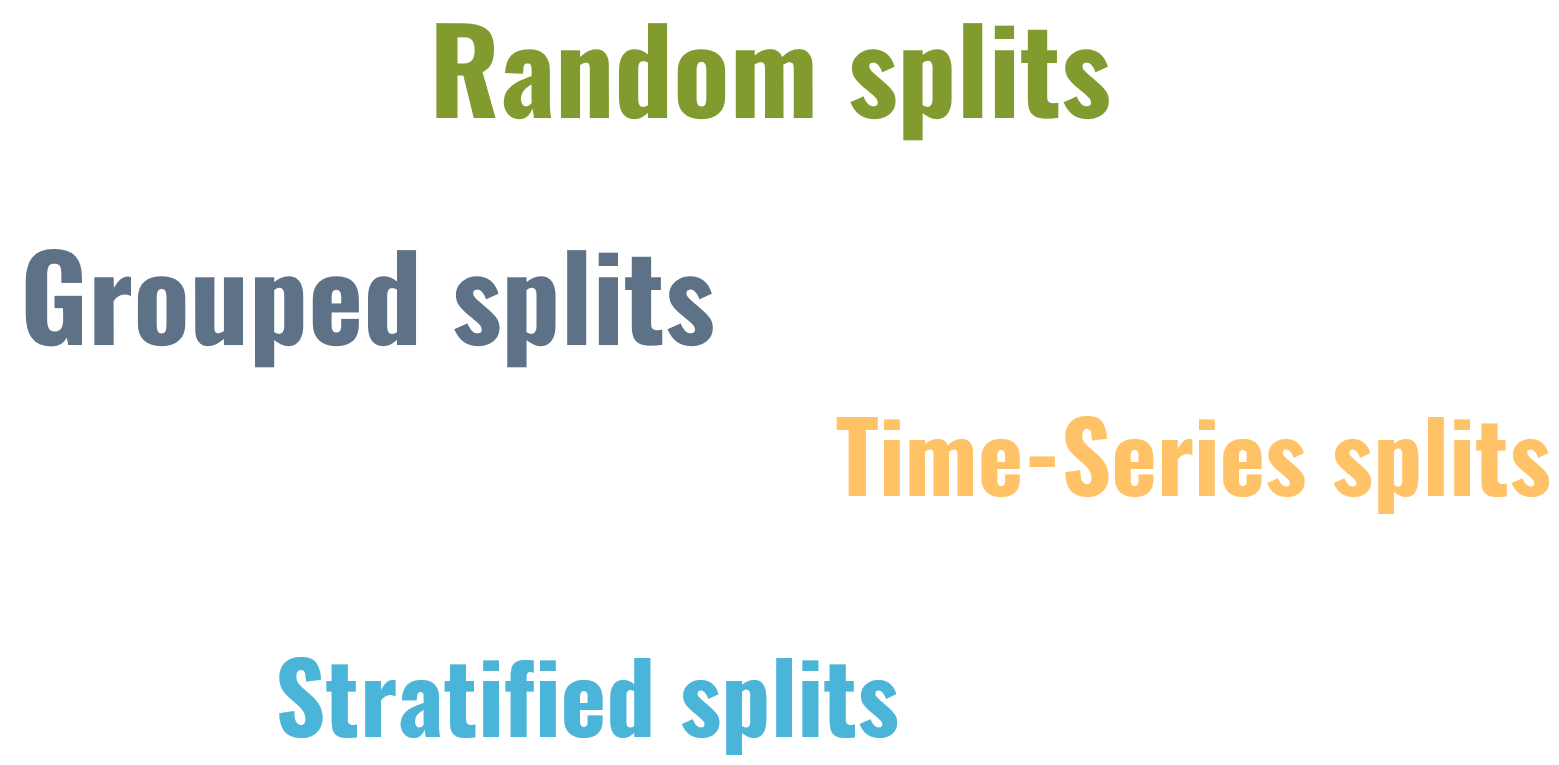
\includegraphics[width=0.8\textwidth]{pics/validation_independent.png}
	\end{figure}
\end{frame}

%=====================================================================
\subsection{Excursion: SQL and Spark}
%=====================================================================

\begin{frame}
	\frametitle{Excursion: SQL and Spark}
	\begin{quotation}
		Data science is 80\% preparing data, 20\% complaining about preparing data.
	\end{quotation}
	
	\vfill
	
	\begin{columns}[onlytextwidth]
		\column{0.5\textwidth}
		\begin{block}{Typical preprocessing steps?}
		\end{block}
		
		\begin{block}{Good moment to learn}
			\begin{itemize}
				\item data structure
				\item meaning of columns
				\item sources of bias
			\end{itemize}
		\end{block}
		
		\column{0.5\textwidth}
		\begin{block}{How to do preprocessing?}
			Data = files on disk or tables in database
			\begin{itemize}
				\item If small $\rightarrow$ R/Python
				\item If large? $\rightarrow$ Database Management System (DBMS) or Spark
				\item Communication via SQL
			\end{itemize}
		\end{block}
	\end{columns}
\end{frame}

\begin{frame}
	\frametitle{SQL}
	\begin{columns}[onlytextwidth]
		\column{0.5\textwidth}
		\begin{block}{Structured Query Language}
			\begin{itemize}
				\item Pronounced?
				\item Important in data science
				\item In DBMS or R/Python
				\item ISO norm $\leftrightarrow$ dialects
				\item SQL queries
			\end{itemize}
		\end{block}
		
		\column{0.5\textwidth}
		\begin{block}{DuckDB (since 2018)}
			\begin{itemize}
				\item In-process, open-source DBMS
				\item Easy to install in R/Python
				\item No dependencies (Java etc.)
				\item Fast
				\item Out-of-core capabilities
			\end{itemize}
		\end{block}
	\end{columns}
	
	\vfill
	
	\begin{exampleblock}{Learn SQL with examples}
		\begin{itemize}
			\item Diamonds (from memory)
			\item Taxi (from Parquet)
		\end{itemize}
	\end{exampleblock}
\end{frame}

\begin{frame}
	\frametitle{Apache Spark}
	\begin{columns}
		\column{0.5\textwidth}
		\begin{itemize}
			\item Distributed, open-source cluster computing system for big data
			\item Apache project since 2013
			\item Heavily used in industry
			\item Written in Scala
			\item Contains SQL engine
			\item Can be used from R/Python
		\end{itemize}
		
		\vfill
		
		\column{0.5\textwidth}
		
		\begin{exampleblock}{Examples}
			\begin{itemize}
				\item Diamonds (from memory)
				\item Taxi (from Parquet)
			\end{itemize}
		\end{exampleblock}
	\end{columns}
\end{frame}

%%=====================================================================
\section{Trees}
%=====================================================================

\begin{frame}
	\frametitle{Outline}
	
	\begin{itemize}
		\item Decision Trees
		\item Random Forests
		\item Gradient Boosted Trees
	\end{itemize}
\end{frame}

%=====================================================================
\subsection{Decision Trees}
%=====================================================================

\begin{frame}
	\frametitle{Decision Trees}
	\begin{columns}[onlytextwidth]
		\column{0.5\textwidth}
		\begin{itemize}
			\item Simple		
			\item Easy to interpret
			\item Decision trees are like wolves:
			
			Weak alone, strong together
			\item Around since 1984 
			
			(Breiman, Friedman)
		\end{itemize}
		
		\column{0.5\textwidth}
		\begin{figure}
			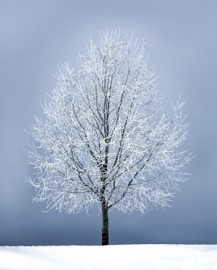
\includegraphics[width=0.7\textwidth]{pics/real_tree.jpg}
			\tiny{https://images.pexels.com/photos/3732527/pexels-photo-3732527.jpeg}
		\end{figure}
	\end{columns}
\end{frame}


\begin{frame}
	\frametitle{What is a Decision Tree?}
	\begin{columns}[onlytextwidth]
		\column{0.5\textwidth}
		\begin{block}{Greedy recursive partitioning}
			\begin{enumerate}
				\item Split: find best ``yes/no'' question on best feature to make total loss smaller
				\item Apply Step 1 recursively
			\end{enumerate}
		\end{block}
		
		\begin{block}{Predictions}
			\begin{itemize}
				\item Follow splits and use leaf value $\gamma_j$
				\item Usually, $\gamma_j$ is average response in leaf $j$
				\item Terminal regions $R_1, \dots, R_J$
				\item $\bx$ falls in leaf $j$ $\Leftrightarrow$ $\bx \in R_j$
				\item $\hat f(\bx) = \sum_{j = 1}^{J} \gamma_j \boldsymbol 1\{\bx \in R_j\}$
			\end{itemize}
		\end{block}
		
		\column{0.45\textwidth}
		\begin{figure}
			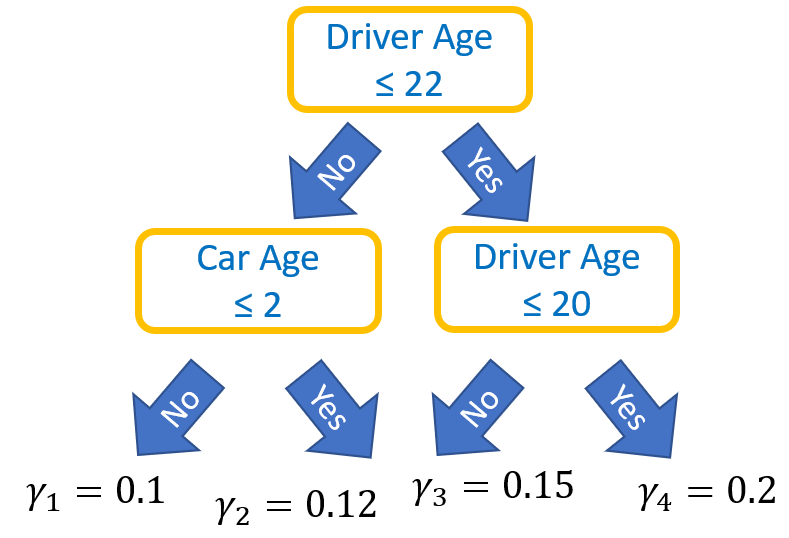
\includegraphics[width=1\textwidth]{../figs/a_tree.png}
		\end{figure}
		\centering The tree does a headstand
		
		\begin{example}
		\end{example}
	\end{columns}
\end{frame}

\begin{frame}
	\frametitle{Properties of Decision Trees}
	
	\begin{columns}[onlytextwidth]
		\column{0.5\textwidth}
		\begin{itemize}
			\item Outliers
			\item Missing values
			\item Categorical covariates
			\item Greedy
		\end{itemize}
		
		\column{0.5\textwidth}	
		\begin{itemize}
			\item Interactions
			\item Extrapolation
			\item Instability
			
			\vphantom{T}
		\end{itemize}
	\end{columns}
	
	\vfill 
	
	Most properties are inherited to groups/ensembles of decision trees
	
	\vfill
	
	From nearest neighbors to decision trees: Short video by Jerome Friedman: \url{https://www.youtube.com/watch?v=8hupHmBVvb0}
\end{frame}

%=====================================================================
\subsection{Random Forests}
%=====================================================================

\begin{frame}
	\frametitle{Random Forests}
	\begin{columns}[onlytextwidth]
		\column{0.5\textwidth}
		\begin{itemize}
			\item Combine many decision trees
			\item Perform very well
			\item Black Box
			\item Around since 2001 (Breiman)
			\item Why is combination of trees better than a single one?
		\end{itemize}
		
		\column{0.5\textwidth}
		\begin{figure}
			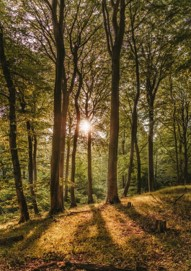
\includegraphics[width=0.6\textwidth]{pics/real_forest.jpg}
			\tiny{https://images.pexels.com/photos/1459534/pexels-photo-1459534.jpeg}
		\end{figure}
	\end{columns}
\end{frame}

\begin{frame}
	\frametitle{Ensembling and Bagging}
	\begin{block}{Ensembling}
		\begin{itemize}
			\item Combine multiple models (\alert{base learners}) to single one
			\item Example: $k$-nearest-neighbor with different $k$
			\item Often out-of-sample performance gain due to lower variance 
			
			$\rightarrow$ diversified stock portfolio
		\end{itemize}
	\end{block}
	
	\begin{block}{Algorithm: Bagging (\alert{B}ootstrap \alert{agg}regat\alert{ing})}
		\begin{enumerate}
			\item Select $B$ bootstrapped training data sets from the original training data
			\item Fit model $\hat f^{*j}(\bx)$ on each of them
			\item Return the bagged model 
			$
			\hat f(\bx) = \frac{1}{B} \sum_{j = 1}^B f^{*j}(\bx)
			$
		\end{enumerate}
	\end{block}
	
	\begin{example}
	\end{example}
\end{frame}

\begin{frame}
	\frametitle{Remarks on Bagging}
	
	\begin{itemize}
		\item Base learners
		\item Out-of-bag (OOB)
		\item Parallel computing
		\item Performance versus complexity
	\end{itemize}
\end{frame}

\begin{frame}
	\frametitle{From Bagging to Random Forests}
	A random forest is a bagged decision tree with an extra twist
	
	\begin{block}{Twist}
		\begin{itemize}
			\item Additional source of randomness
			\item Each split considers only random feature subset (often $p/3$ or $\sqrt p$)
			\item Additional decorrelation $\rightarrow$ stronger diversification
		\end{itemize}
	\end{block}
	
	\begin{block}{Algorithm: Random forest (regression)}
		\begin{enumerate}
			\item Select $B$ bootstrapped training data sets from the original training data
			\item Fit (usually deep) decision tree $\hat f^{*j}(\bx)$ on each of them. For each split, consider only random feature subset
			\item Return the random forest
			$
			\hat f(\bx) = \frac{1}{B} \sum_{j = 1}^B f^{*j}(\bx)
			$
		\end{enumerate}
	\end{block}
\end{frame}

\begin{frame}
	\frametitle{Comments on Random Forests}
	
	\begin{itemize}
		\item Number of trees
		\item Deep trees and diversification 
		\item Don't trust performance on the training set
		\item Parameter tuning
	\end{itemize}
	
	\vfill
	
	Regarding \alert{parameter tuning}: Short video by Adele Cutler on working with Leo Breiman: \url{https://www.youtube.com/watch?v=t8ooi_tJHSE}
	
	\vfill
	
	\begin{example}
	\end{example}
\end{frame}

\begin{frame}
	\frametitle{Interpreting a Black Box}
	\begin{columns}
		\column{0.3\textwidth}
		\begin{block}{Study for each model}
			\begin{enumerate}
				\item Performance
				\item Variable importance
				\item Effects
			\end{enumerate}
		\end{block}
		\column{0.7\textwidth}
		\begin{block}{XAI}
			\begin{itemize}
				\item e{\bf X}plainable {\bf A}rtificial {\bf I}ntelligence
				\item Collection of methods to interpret models
				\item Examples: Split-gain importance, ICE, PDP
			\end{itemize}
		\end{block}
	\end{columns}
	
	\vfill
	
	\begin{example}
		\begin{itemize}
			\item Split gain importance of random forest
			\item Variable importance and linear regression?
		\end{itemize}
	\end{example}
\end{frame}

\begin{frame}
	\frametitle{Individual Conditional Expectation (ICE)}
	\begin{block}{Basic thinking}
		\begin{itemize}
			\item In \alert{additive} linear model $f$, the effect of $X^{(j)}$ is fully described by its coefficient(s)
			\item It describes how $f$ reacts on changes in $X^{(j)}$ (Ceteris Paribus)
			\item What if model involves complex interactions?
		\end{itemize}
	\end{block}
	
	\begin{block}{Idea (Goldstein et al., 2015)}
		\begin{itemize}
			\item Study (Ceteris Paribus) effect of $X^{(j)}$ for \alert{one} observation
			\item {\em ICE function} for feature $X^{(j)}$ of model $f$ and observation $\bx \in \R^p$
			$$
			\text{ICE}_j: v \in {\R} \mapsto f(v, \bx_{\setminus j})
			$$
			\item $\bx_{\setminus j}$ denotes all but the $j$-th component of $\bx$, which is replaced by $v$
			\item {\em ICE curve} represents graph $(v, \text{ICE}_j(v))$ for grid of values $v \in \R$
		\end{itemize}
	\end{block}
\end{frame}

\begin{frame}
	\frametitle{ICE Plot: Visualize ICE Curves of many Observations}
	\begin{example}
	\end{example}
	
	\begin{columns}[onlytextwidth]
		\column{0.5\textwidth}
		\begin{block}{Notes}
			\begin{itemize}
				\item Curves with different shapes indicate interaction effects
				\item Parallel curves $\Leftrightarrow$ additivity in $X^{(j)}$
				\item Centered ICE plots
				\item Usually on link scale (why?)
			\end{itemize}
		\end{block}
		
		\column{0.5\textwidth}
		\begin{alertblock}{Pros and Cons}
			\begin{itemize}
				\item[+] Simple to compute
				\item[+] Easy to interpret (Ceteris Paribus)
				\item[+] Gives impression about interactions
				\item[--] Ceteris Paribus can be unnatural
				\item[--] Model applied to rare/impossible $\bx$
			\end{itemize}
		\end{alertblock}
	\end{columns}
\end{frame}

\begin{frame}
	\frametitle{Partial Dependence Plot PDP (Friedman 2001)}
	\begin{itemize}
		\item Average of many ICE curves
		\item Ceteris Paribus effect of $X^{(j)}$ averaged over all interaction effects
		\item (Empirical) partial dependence function of $j$-th feature
		$$
		\text{PD}_j(v) = \frac{1}{n} \sum_{i = 1}^n \hat f(v, \bx_{i,\setminus j})
		$$
		\item $\bx_{i,\setminus j}$ feature vector of $i$-th observation without $j$-th component
		\item PDP equals graph $(v, \text{PD}_j(v))$ for grid of values $v \in \R$
		\item Sum runs over reference data (=?)
		\item Pros/cons similar to ICE, but no info on interaction
	\end{itemize}
	
	\vfill 
	
	\begin{example}
	\end{example}
\end{frame}

%=====================================================================
\subsection{Gradient Boosted Trees}
%=====================================================================

\begin{frame}
	\frametitle{Gradient Boosted Trees}
	\begin{columns}[onlytextwidth]
		\column{0.5\textwidth}
		\begin{itemize}
			\item Combine many decision trees
			\item Perform very well
			\item Black Box
			\item Around since 2001 (Friedman)
			\smash{\raisebox{.6\dimexpr3\baselineskip+0\itemsep+5\parskip}{$\left.\rule{0pt}{.6\dimexpr4\baselineskip+0\itemsep+6\parskip}\right\}\text{\rotatebox[origin=c]{90}{\footnotesize \alert{Like random forests}}}$}}
		\end{itemize}
		
		\column{0.5\textwidth}
		\begin{figure}
			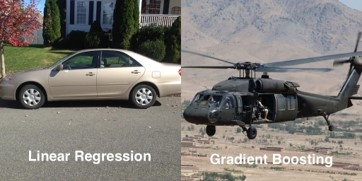
\includegraphics[width=0.95\textwidth]{pics/helicopter.jpg}
			\tiny{https://www.gormanalysis.com/blog/gradient-boosting-explained/}
		\end{figure}
	\end{columns}
\end{frame}

\begin{frame}
	\frametitle{Boosting}
	\begin{block}{Basic idea of boosting (e.g. Schapire, 1990)}
		\begin{enumerate}
			\item Fit simple model $\hat f$ to data
			\item For $k = 1, \dots, K$ do:
			\begin{itemize}
				\item[a.] Find simple model $\hat f^k$ that corrects the mistakes of $\hat f$
				\item[b.] Update: $\hat f \leftarrow \hat f + \hat f^k$
			\end{itemize}
		\end{enumerate}
	\end{block}
	
	\begin{block}{How to find updates $\hat f^k$?}
		Use decision trees $\rightarrow$ \alert{boosted trees}
		\begin{itemize}
			\item Use reweighting heuristic for binary classification
			
			$\rightarrow$ AdaBoost (Freund and Schapire, 1995)
			\item Reduce total loss $Q(\hat f + \hat f^k) = \sum_{i = 1}^n L(y_i, \hat f(\bx_i) + \hat f^k (\bx_i))$ 
			
			$\rightarrow$ \alert{Gradient boosting} (Friedman, 2001)
		\end{itemize}
	\end{block}
\end{frame}

\begin{frame}
	\frametitle{Gradient Descent}
	\begin{columns}[onlytextwidth]
		\column{0.45\textwidth}
		\begin{block}{Minimize function $h: \R^n \to \R$}
			\begin{enumerate}
				\item Start at some value $\hat x$
				\item Repeat: $\hat x \leftarrow \hat x - \lambda g$
			\end{enumerate}
			\begin{itemize}
				\item $\lambda$: Step size or learning rate
				\item Gradient of $h$ at $\hat x$:
				$$
				g = \left[\frac{\partial h(x)}{\partial x}\right]_{x = \hat x}
				$$ 
				\item $g$ points in direction of steepest ascent
			\end{itemize}
		\end{block}
		
		\column{0.55\textwidth}
		\begin{figure}
			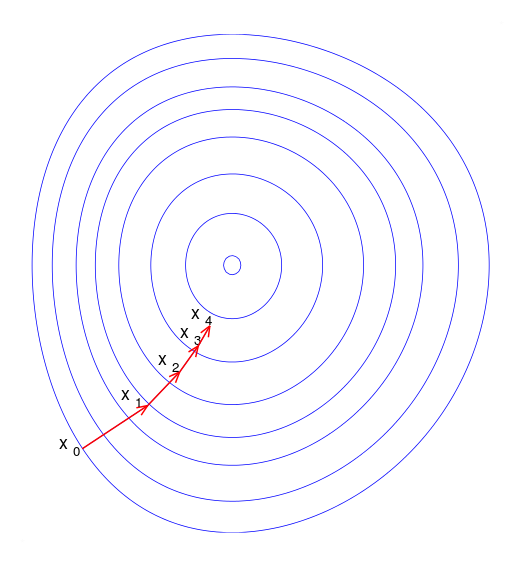
\includegraphics[width=0.8\textwidth]{../figs/gradient_descent.png}
			\tiny\url{https://en.wikipedia.org/wiki/Gradient_descent}
		\end{figure}
	\end{columns}
\end{frame}

\begin{frame}
	\frametitle{Gradient Boosting}
	\begin{columns}[onlytextwidth]
		\column{0.5\textwidth}
		\begin{block}{Gradient descent of $Q(f)$}
			\begin{itemize}
				\item $Q(f) = \sum_{i = 1}^n L(y_i, f(\bx_i))$
				\item $f = \left(f(\bx_1), \dots, f(\bx_n)\right) \in \R^n$
			\end{itemize}
			
			\begin{enumerate}
				\item Start at some value $\hat f$
				\item Repeat: $\hat f \leftarrow \hat f - \lambda g$ with
				$$
				g = \left[\frac{\partial Q(f)}{\partial f}\right]_{f = \hat f}
				$$
				having components
				$$
				g_i = \left[\frac{\partial L(y_i, f(\bx_i))}{\partial f(\bx_i)}\right]_{f(\bx_i) = \hat f(\bx_i)}
				$$
			\end{enumerate}
		\end{block}
		
		\column{0.5\textwidth}
		\begin{block}{For squared error?}
			\begin{itemize}
				\item $L(y, z) = (y-z)^2/2$
				\item Plugging in:
				$
				g_i = -(\underbrace{y_i - \hat f(\bx_i)}_{\text{Residual } r_i})
				$
				\item Repeat: $\hat f(\bx_i) \leftarrow \hat f(\bx_i) + \underbrace{\lambda r_i}_{\hat f^k \text{?}}$
			\end{itemize}
		\end{block}
		\begin{block}{Boosting with $\hat f^k = -\lambda g_i$? Now way\dots} 
			\begin{enumerate}
				\item $y_i$ unknown in application
				\item Should work for all $\bx$
			\end{enumerate}
			$\rightarrow$ replace $-g_i$ by predictions of tree
		\end{block}
	\end{columns}
\end{frame}

\begin{frame}
	\frametitle{Gradient Boosted Trees for Squared Error Loss}
	\begin{block}{Algorithm}
		\begin{enumerate}
			\item Initialize $\hat f(\bx) = \frac{1}{n}\sum_{i = 1}^{n} y_i$
			\item For $k = 1, \dots, K$ do:
			\begin{enumerate}
				\item[a.] For $i = 1, \dots, n$, calculate residuals $r_i = y_i - \hat f(\bx_i)$
				\item[b.] Model the $r_i$ as a function of the $\bx_i$ by fitting a regression tree $\hat f^k$
				\item[c.] Update: $\hat f(\bx) \leftarrow \hat f(\bx) + \lambda \hat f^k(\bx)$
			\end{enumerate}
			\item Output $\hat f(\bx)$
		\end{enumerate}
	\end{block}
	
	\begin{block}{General loss functions?}
		\begin{itemize}
			\item Replace residuals by negative gradients of loss function
			\item Leaf values might be suboptimal $\rightarrow$ replace by optimal values
		\end{itemize}
	\end{block}
\end{frame}

\begin{frame}
	\frametitle{Gradient Boosted Trees for General Losses}
	\begin{enumerate}
		\item Initialize $\hat f(\bx) = \text{argmin}_\gamma \sum_{i = 1}^{n} L(y_i, \gamma)$
		\item For $k = 1, \dots, K$ do:
		\begin{enumerate}
			\item[a.] For $i = 1, \dots, n$, calculate negative gradients (pseudo-residuals)
			$$
			r_i = -\left[\frac{\partial L(y_i, f(\bx_i))}{\partial f(\bx_i)}\right]_{f(\bx_i) = \hat f(\bx_i)}
			$$
			\item[b.] Model $r_i$ as function of $\bx_i$ by regression tree $\hat f^k$ with terminal regions $R_1, \dots, R_J$
			\item[c.] For each $j = 1, \dots, J$, use line-search to find the optimal leaf value 
			$$
			\gamma_j = \text{argmin}_{\gamma} \sum_{\bx_i \in R_j} L(y_i, \hat f(\bx_i) + \gamma)
			$$
			\vspace{-1em}
			\item[d.] Update: $\hat f(\bx) \leftarrow \hat f(\bx) + \lambda \underbrace{\sum_{j = 1}^{J} \gamma_j \boldsymbol 1\{\bx \in R_j\}}_{\text{modified tree}}$
		\end{enumerate}
		\item Output $\hat f(\boldsymbol x)$
	\end{enumerate}
\end{frame}

\begin{frame}
	\frametitle{Remarks}
	\begin{itemize}
		\item Predictions are sum of short decision trees (with modified leaf values)
		\item Random forest: average of deep trees
		\item How to select learning rate $\lambda$, number of trees $K$, \dots?
		\item (AdaBoost is gradient tree boosting with exponential loss)
	\end{itemize}
\end{frame}

\begin{frame}
	\frametitle{Modern Implementations}
	\begin{columns}[onlytextwidth]
		\column{0.5\textwidth}
		\begin{block}{Timeline}
			\begin{enumerate}
				\item XGBoost (2014)
				\item LightGBM (2016)
				\item CatBoost (2017)
			\end{enumerate}
		\end{block}
		
		\column{0.5\textwidth}
		\begin{block}{Differences to Friedman's original}
			\begin{itemize}
				\item Use of second order gradients 
				
				$\rightarrow$ no line-search necessary
				\item Histogram binning
				
				$\rightarrow$ speeds up tree growth
				
				\item Penalized objective function
			\end{itemize}
		\end{block}
	\end{columns}
	\vfill
	
	\begin{example}
	\end{example}
\end{frame}

\begin{frame}
	\frametitle{Parameter Tuning is Essential}
	\begin{columns}[onlytextwidth]
		\column{0.7\textwidth}
		\begin{enumerate}
			\item Number of boosting rounds/trees  $K$
			
			$\rightarrow$ find by early stopping (validation/CV)
			\item Learning rate $\lambda$
			
			$\rightarrow$ to get reasonable number of rounds
			\item Regularization
			\begin{itemize}
				\item Tree depth, number of leaves, loss penalties, etc.
				\item $\rightarrow$ Grid/Randomized search and iterate process
			\end{itemize}
		\end{enumerate}
		\column{0.3\textwidth}
		\begin{block}{Comments}
			\begin{itemize}
				\item Why not one big grid search on all parameters?
				\item Objective/metrics
			\end{itemize}
		\end{block}
	\end{columns}
	
	\vfill
	
	\begin{example}
		\begin{itemize}
			\item XGBoost
			\item LightGBM
		\end{itemize}
	\end{example}
\end{frame}

%=====================================================================
\section{Neural Nets}
%=====================================================================

\begin{frame}
	\frametitle{Outline}
	
	\begin{itemize}
		\item Understanding Neural Nets
		\item Practical Considerations
		\item Extended examples
	\end{itemize}
\end{frame}

\begin{frame}
	\frametitle{Neural Nets}
	\begin{itemize}
		\item Around since the 1950ies
		\item Underwent different development steps, e.g.
		\begin{itemize}
			\item use of backpropagation
			\item GPUs
		\end{itemize}
		\item Black Box
		\item TensorFlow/Keras, PyTorch
	\end{itemize}
\end{frame}

\begin{frame}
	\frametitle{``Swiss Army Knife'' among ML Algorithms}
	\begin{figure}
		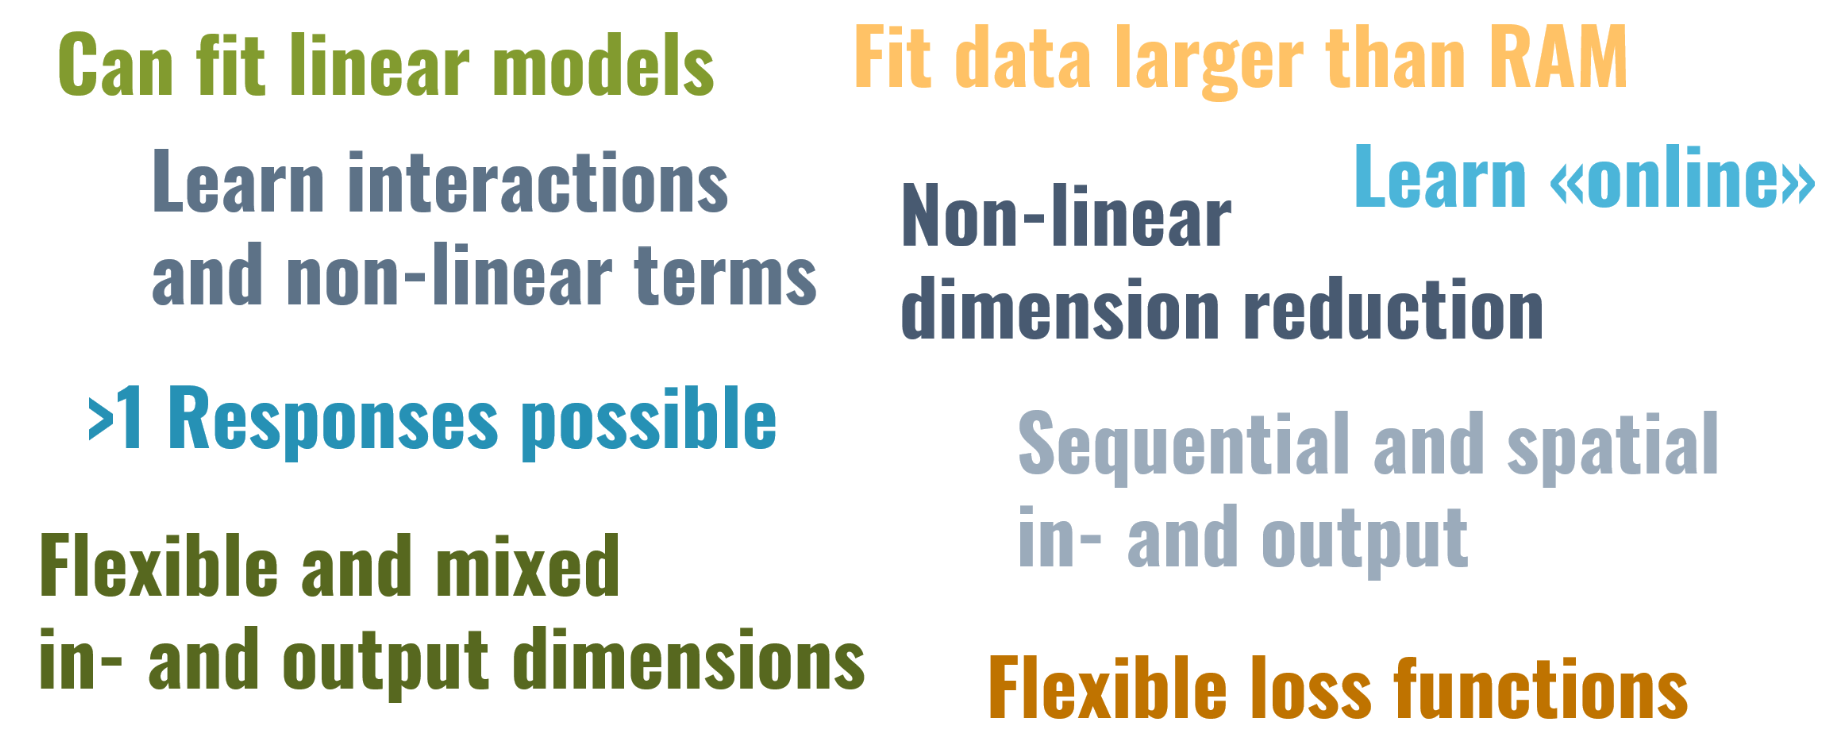
\includegraphics[width=0.9\textwidth]{pics/nn_knife.png}
	\end{figure}
\end{frame}

%=====================================================================
\subsection{Understanding Neural Nets}
%=====================================================================

\begin{frame}
	\frametitle{Understanding Neural Nets in three Steps}
	\begin{enumerate}
		\item Linear regression as neural net
		\item Hidden layers
		\item Activation functions
	\end{enumerate}
	
	\vfill
	
	Using \alert{diamonds} data
\end{frame}

\begin{frame}
	\frametitle{Step 1: Linear Regression as Neural Net}
	\begin{columns}
		\column{0.35\textwidth}
		\begin{itemize}
			\item $\E(\text{price})=\alpha+\beta \cdot \text{carat}$
			\item OLS 
			
			$\hat\alpha \approx -2256$, $\hat\beta \approx 7756$
			\item Represented as neural network graph
		\end{itemize}
		\column{0.65\textwidth}
		\begin{figure}
			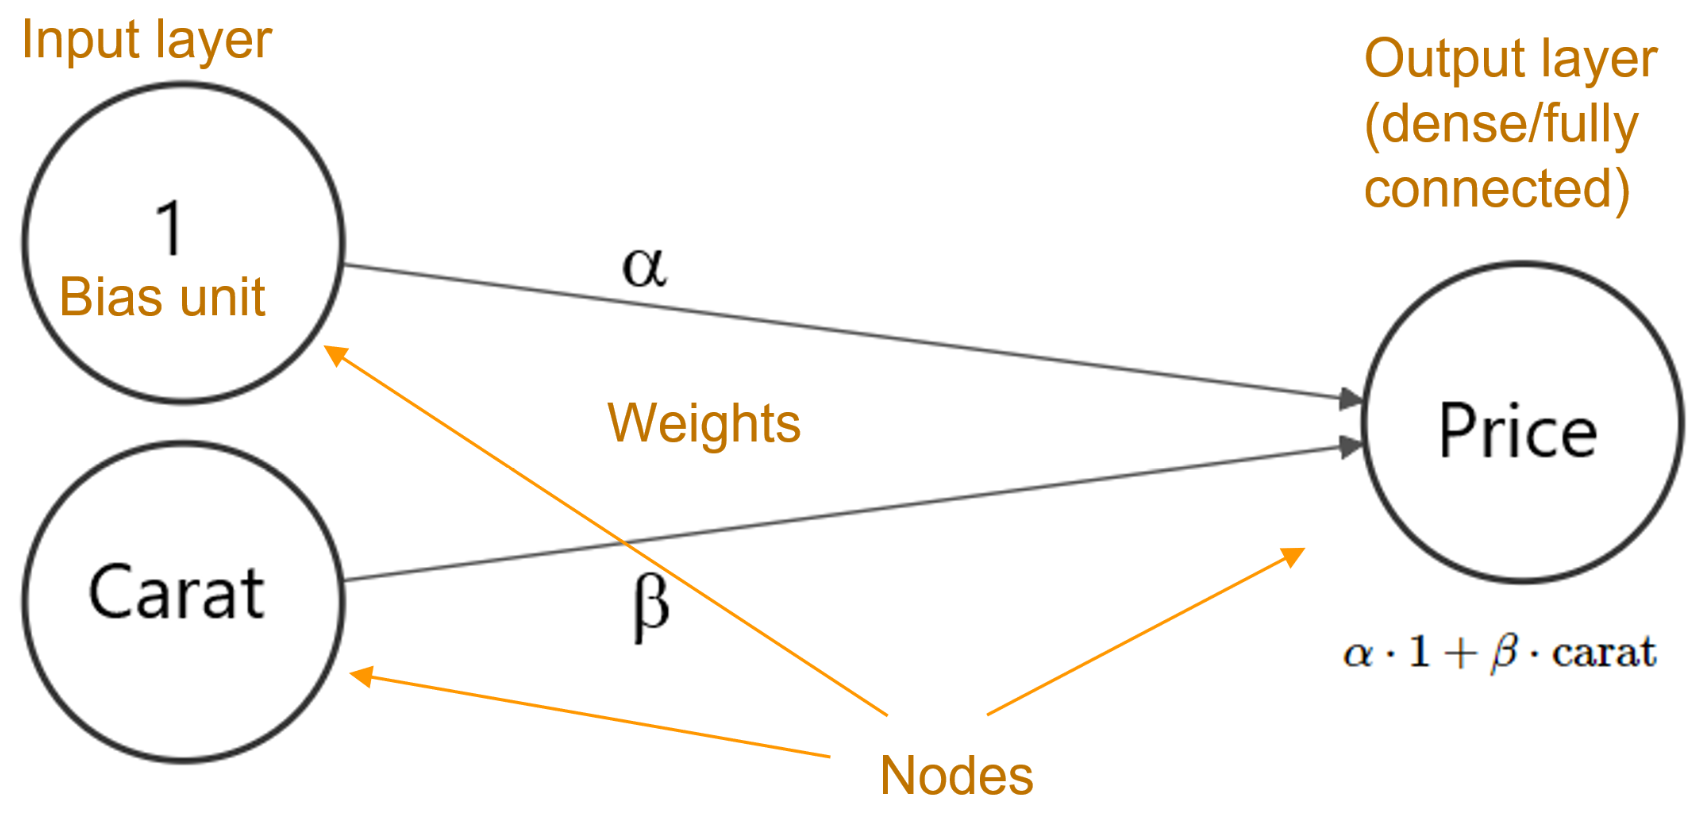
\includegraphics[width=0.9\textwidth]{pics/simple_nn.png}
		\end{figure}
	\end{columns}
	
	\vfill
	
	\begin{exampleblock}{\centering Example}
	\end{exampleblock}
\end{frame}

\begin{frame}
	\frametitle{The Optimization Algorithm}
	\begin{block}{Mini-batch gradient descent with backpropagation}
		Notation: Neural net $f_\beta$; its total loss on data $D$ and loss function $L$: 
		\vspace{-0.5em}
		$$
		Q(f_\beta, D) = \sum_{(y_i, \boldsymbol x_i) \in D} L(y_i, f_\beta(\boldsymbol x_i))
		$$
		\vspace{-1.2em}
		\begin{enumerate}
			\item Init: Randomly initialize parameter vector $\beta$ by $\hat \beta$
			\item Forward: Calculate $Q(f_{\hat\beta}, D_\text{batch})$ on \alert{batch}
			\item Backprop: Modify $\hat \beta$ to improve $Q(f_{\hat\beta}, D_\text{batch})$ 
			\begin{enumerate}
				\item Calculate partial derivatives $\nabla \hat \beta = \frac{\partial Q(f_\beta, D_\text{batch})}{\partial \beta}\mid_{\beta = \hat \beta}$ using backprop (=?)
				\item Gradient descent: Move slightly into right direction: $\hat \beta \leftarrow \hat \beta  - \lambda \cdot \nabla \hat \beta$
			\end{enumerate}
			\item Repeat Steps 2 and 3 until one \alert{epoch} is over
			\item Repeat Step 4 until some stopping criterion triggers
		\end{enumerate}
	\end{block}
	
	SGD? Local minima?
\end{frame}

\begin{frame}
	\frametitle{Step 2: Hidden Layers}
	\begin{columns}
		\column{0.33\textwidth}
		\begin{itemize}
			\item Add \alert{hidden layers} for more parameters 
			
			(= flexibility)
			\item Their nodes are latent/implicit variables
			\item Representational learning
			\item \small{\alert{Encoding}?}
			\item \small{\alert{Deep} neural net?}
		\end{itemize}
		\begin{example}
		\end{example}
		\column{0.67\textwidth}
		\begin{figure}
			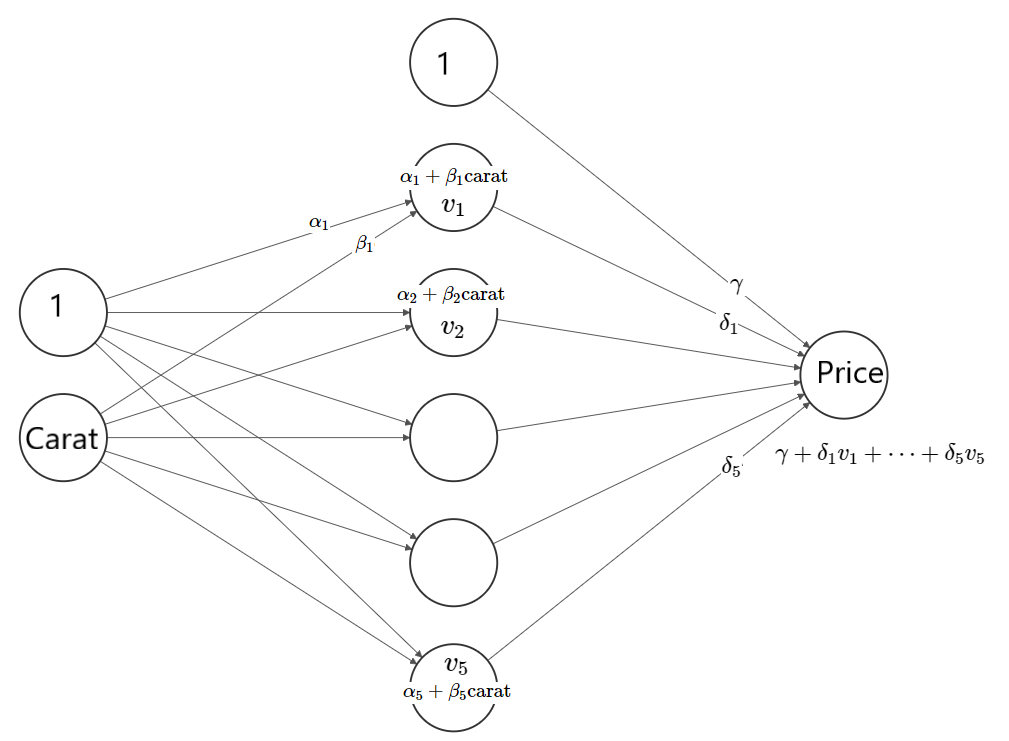
\includegraphics[width=0.98\textwidth]{../figs/nn_1_hidden.png}
		\end{figure}
	\end{columns}
\end{frame}

\begin{frame}
	\frametitle{Step 3: Activation Functions}
	Non-linear transformations $\sigma$ of node values necessary!
	\begin{columns}[onlytextwidth]
		\column{0.35\textwidth}
		\begin{itemize}
			\item tanh: $\sigma(x) = \frac{e^x - e^{-x}}{e^x + e^{-x}}$
			\item ReLU: $\sigma(x) = \text{max}(0, x)$
		\end{itemize}
		\begin{figure}
			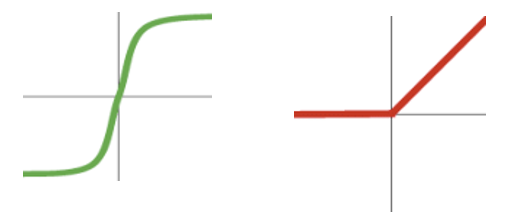
\includegraphics[width=0.8\textwidth]{pics/activation_functions.png}
		\end{figure}
		\begin{block}{Two purposes}
			\begin{itemize}
				\item Imply interactions and non-linear terms
				\item Inverse link as in GLMs
			\end{itemize}
		\end{block}
		\begin{example}
		\end{example}
		\column{0.65\textwidth}
		\begin{figure}
			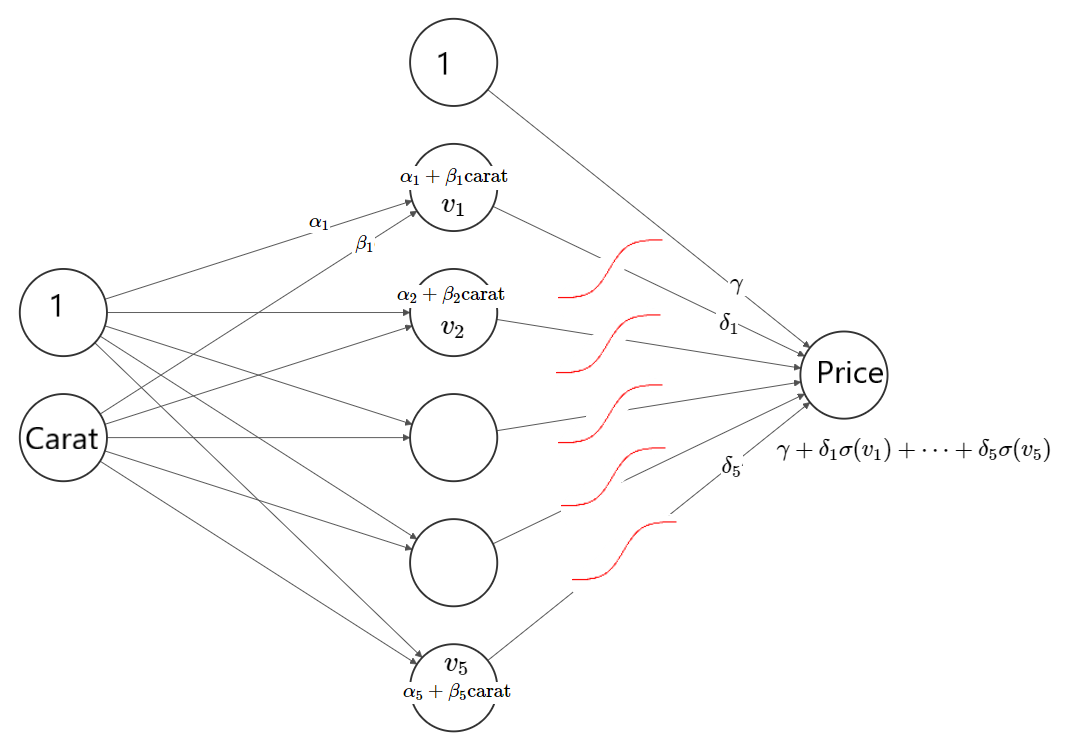
\includegraphics[width=0.98\textwidth]{../figs/nn_activation.png}
		\end{figure}
	\end{columns}
\end{frame}

%=====================================================================
\subsection{Practical Consideration}
%=====================================================================

\begin{frame}
	\frametitle{Practical Considerations}
	\begin{figure}
		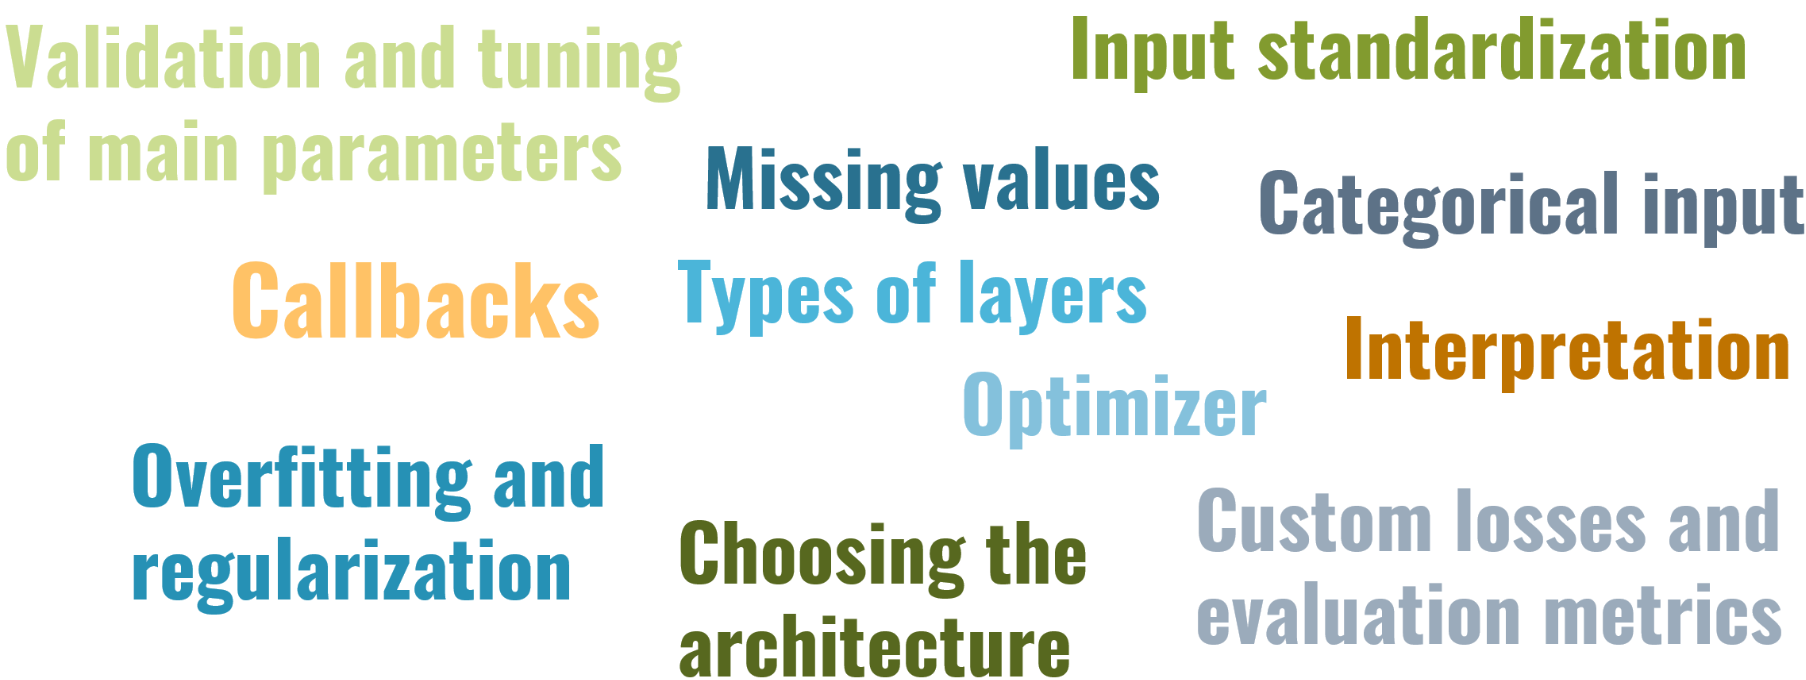
\includegraphics[width=0.9\textwidth]{pics/nn_practical.png}
	\end{figure}
\end{frame}

%=====================================================================
\subsection{Extended Examples}
%=====================================================================

\begin{frame}
	\frametitle{Example: Diamonds}
	\begin{figure}
		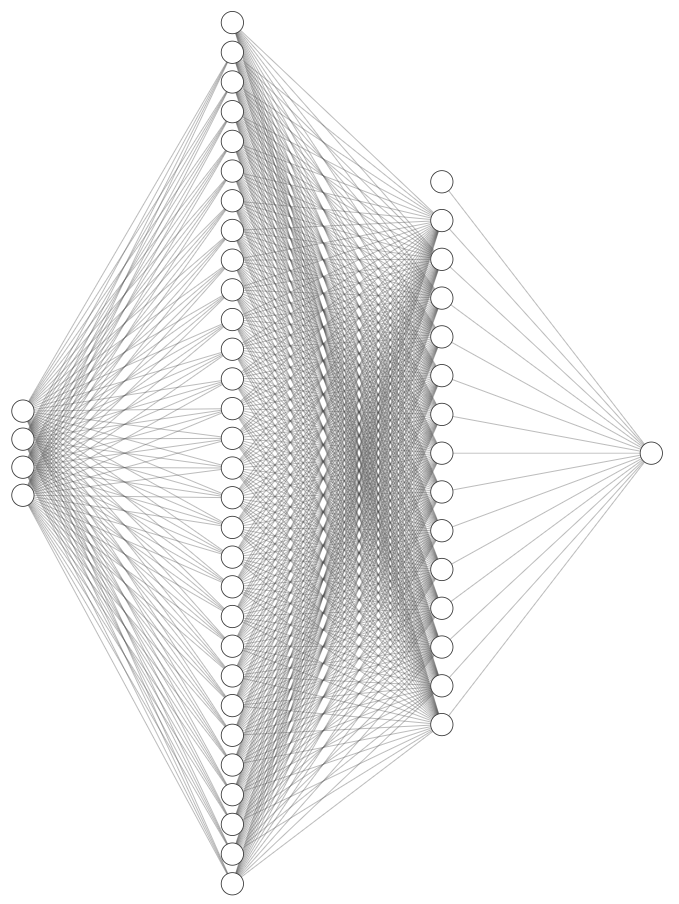
\includegraphics[width=0.6\textheight]{../figs/nn_2_hidden.png}
	\end{figure}
\end{frame}

\begin{frame}
	\frametitle{Excursion: Model-Agnostic Importance Measure}
	\alert{Permutation importance} of feature $X^{(j)}$, data $D$, and performance measure $S$:
	$$
	\text{PVI}(j, D) = S(\hat f, D^{(j)}) - S(\hat f, D)
	$$
	\vspace{-1.5em}
	\begin{itemize}
		\item $D^{(j)}$ is version of $D$ with randomly permuted values in $j$-th feature column
		\item Read: How much $S$ worsens after shuffling column $j$? 
		
		The larger, the more important. If 0, feature is unimportant
		\item Computationally cheap $\rightarrow$ repeat $m$ times
		\item Model is never refitted
		\item Training or test data?
	\end{itemize}
	
	\vfill
	
	\begin{example}
	\end{example}
\end{frame}

\begin{frame}
	\frametitle{Embeddings}
	Represent unordered categorical $X$ with $K$ levels by $m << K$ numeric features
	
	\vfill
	
	\begin{block}{Embedding layer}
		\begin{itemize}
			\item $X$ integer encoded
			\item Dummy matrix $\tilde X$ with $K$ columns
			\item Multiply $\tilde X$ with $(K \times m)$ matrix $\beta$
			\item Embedding matrix $\beta$ estimated like other parameters
			\item Trick: $\tilde X \beta$ is calculated via index slicing from $X$ and $\beta$
			
			$\rightarrow \tilde X$ is never materialized
		\end{itemize}
	\end{block}
	
	\vfill
	
	\begin{example}
		Taxi trips
	\end{example}
\end{frame}

%=====================================================================
\subsection{Excursion: Analysis Scheme X}
%=====================================================================

\begin{frame}
	\frametitle{Excursion: Analysis Scheme X}
	$T(Y)$: quantity of interest
	
	\vfill
	
	\begin{block}{Steps}
		\begin{enumerate}
			\item Calculate $T(Y)$ on the full data
			\item Calculate $T(Y)$ stratified by covariates $X^{(j)}$ $\rightarrow$ bivariate associations
			\item Accompany Step 2 by ML model $\rightarrow$ multivariate associations
			\begin{itemize}
				\item Study model performance
				\item Study variable importance $\rightarrow$ sort results of Step 2
				\item Study PDP (or similar) for each $X^{(j)}$ and compare with Step 2
			\end{itemize}
		\end{enumerate}
	\end{block}
	
	\vfill
	
	\begin{example}
	\end{example}
\end{frame}

%=====================================================================
\subsection{Outro}
%=====================================================================

\begin{frame}
	\frametitle{Comparison of ML Algorithms}
	\begin{figure}
		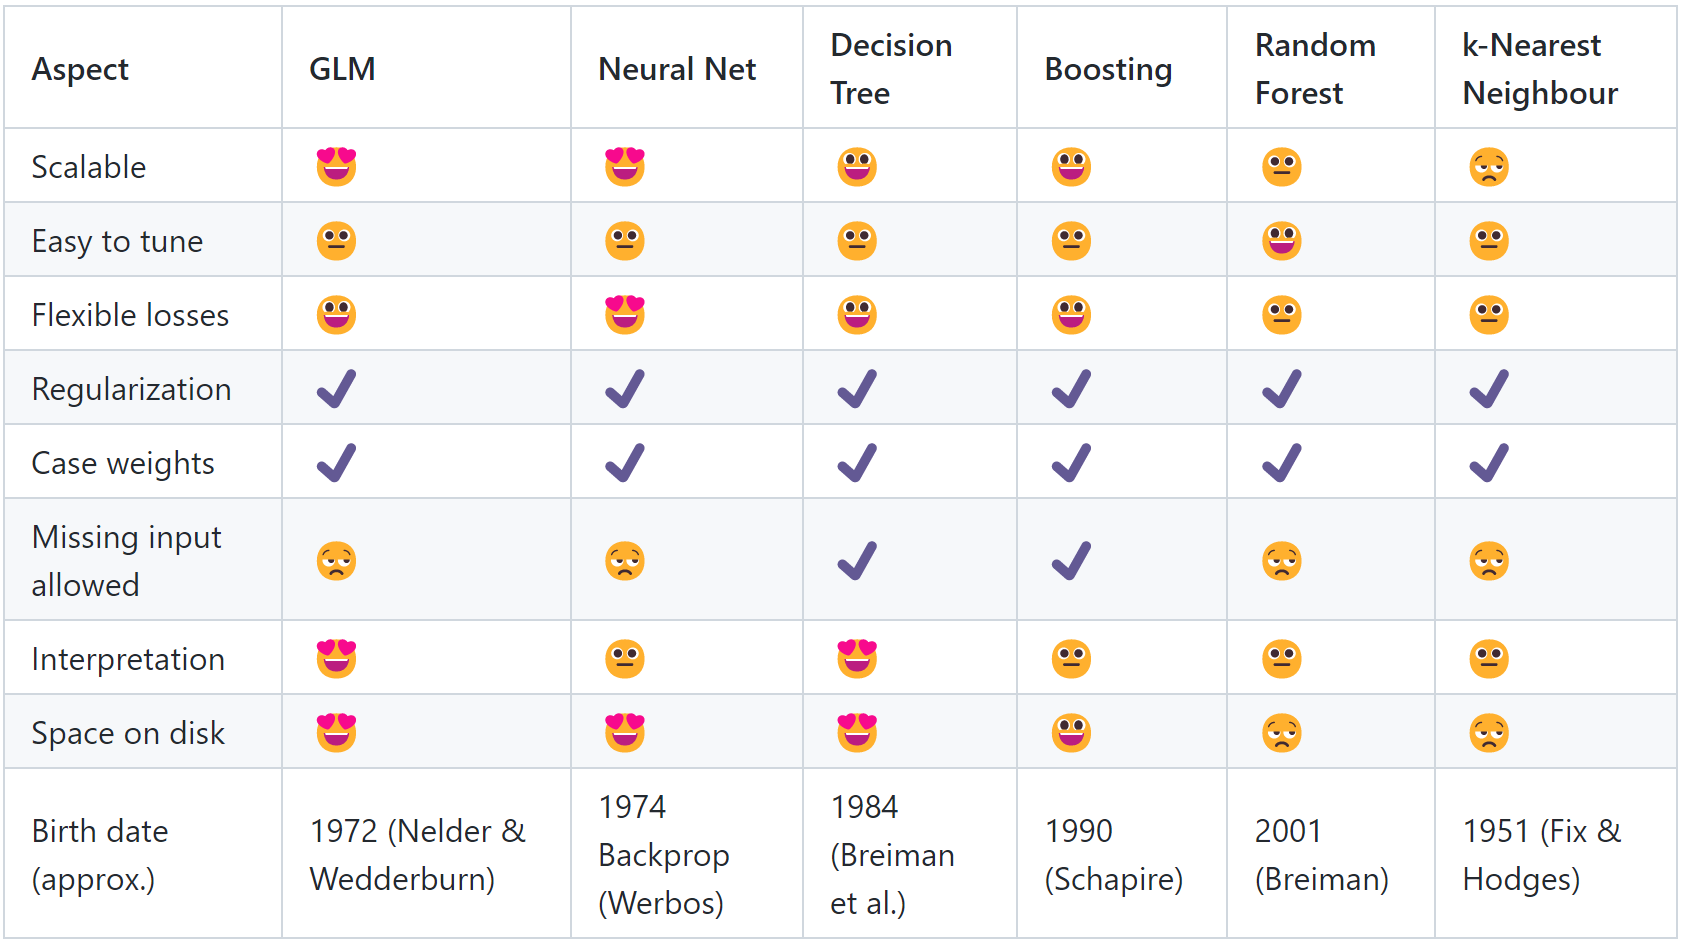
\includegraphics[width=0.9\textwidth]{pics/algorithms.png}
	\end{figure}
\end{frame}

%=====================================================================
\end{document}
%=====================================================================